\documentclass[11pt,a4paper,parskip]{scrartcl}
%%%%%%%%%%%%%%%%%%%%%Packages
\usepackage[utf8x]{inputenc} 
\usepackage{amsfonts} 
\usepackage{amssymb} 
\usepackage{lmodern} 
\usepackage{hyperref} 
\usepackage[ngerman]{babel} 
\usepackage{verbatim} 

%%%%%%%%%%%%%%%%%%%%%%%%%%%%%% Einbindnen Bilder
\usepackage{pdfpages}   %Pdf
\usepackage{graphicx}   %Bilder
\usepackage{svg}        %SVG

%%%%%%%%%%%%%%%%%%%%%%%%%%%%%% Mathe
\usepackage{amsmath} 

%%%%%%%%%%%%%%%%%%%%%%%%%%%%%% Linenumbers 
\usepackage{lineno}
%Tikz Beginn
    \usepackage{tikz} 
    \usepackage{pgfplots}
    \pgfplotsset{compat=1.15}
    %%%%%%%%%%%%%%%%%%%%% - Farben
    \definecolor{class1}{RGB}{228,26,28}
    \definecolor{class2}{RGB}{55,126,184}
    \definecolor{class3}{RGB}{77,175,74}
    \definecolor{class4}{RGB}{152,78,163}
    \definecolor{class5}{RGB}{255,127,0}
    %%%%%%%%%%%%%%%%%%%%%%%%% - Formen
    \tikzset{wagon/.style={draw = gray, ultra thick, opacity = 0.7}}
    \tikzset{class1/.style={draw = class1, ultra thick, opacity = 1}}
    \tikzset{class2/.style={draw = class2, ultra thick, opacity = 1}}
    \tikzset{class3/.style={draw = class3, ultra thick, opacity = 1}}
    \tikzset{class4/.style={draw = class4, ultra thick, opacity = 1}}
    \tikzset{class5/.style={draw = class5, ultra thick, opacity = 1}}
    \tikzset{annotation/.style={draw = black, thick, opacity = 0.7}}
%Tikz Ende
%%%%%%%%%%%%%%%%% Glossar Abkürzungsverzeichnis Beginn
    \usepackage[acronym]{glossaries} %Glossar %\usepackage[acronym, toc]{glossaries} %Glossar mit Aufruf im Inhaltsverzeichnis
    \makeglossaries
    \newglossaryentry{Ablaufberg}{
    name=Ablaufberg,
    description={Der Ablaufberg ist ein in der Regel künstlich angelegter Hügel, über den ein Gleis verläuft. Ablaufberge dienen beim Abdrücken dem Ablaufen lassen von Güter- wagen, die auf diese Weise nach ihren Bestimmungsorten sortiert werden}
}
\newglossaryentry{Bremsprobe}{
    name=Bremsprobe,
    description={Eine Bremsprobe  ist ein zur Vorbereitung von Zugfahrten gehörender Vorgang, bei dem die Funktionsfähigkeit des Bremssystems der Fahrzeuge im Zugverband überprüft wird. Dabei wird im Stillstand das Anlegen und Lösen der zu prüfenden Bremsen kontrolliert}
}
\newglossaryentry{Eisenbahnverkehrsunternehmen}{
    name=Eisenbahnverkehrsunternehmen,
    description={Eisenbahnverkehrsunternehmen sind Eisenbahnen, die Eisenbahnverkehrsleistungen erbringen. \acrshort{EVU}s müssen in der Lage sein, die Zugförderung (Traktion) sicherzustellen\cite{rennsteigbahn}}
}
\newglossaryentry{Heisslaeuferortungsanlage}{
    name=Hei\ss l\" auferortungsanlage,
    description={Eine Heißläuferortungsanlage dient dazu, eine unzulässige Er- wärmung von Radsatzlagern durch Defekte bei Schienenfahrzeugen (sogenannte Heiß- läufer) rechtzeitig feststellen zu können}
}
\newglossaryentry{ep-Bremsen}{
    name=ep-Bremse,
    description={Die elektropneumatische Bremse (ep-Bremse) ist eine durch elektropneumatische Bauteile gesteuerte automatische Druckluftbremse bei Eisenbahnen. Die ep-Bremse ermöglicht das gleichzeitige Bremsen oder Lösen aller Fahrzeuge unabhängig von der Länge des Zuges}
}
\newglossaryentry{ep-assist-Bremsen}{
    name=ep-Assist,
    description={ep-Assist ist die Funktion des ep-Bremsen. Die Funktion beschränkt sich auf das unterstützte Bremsen der \gls{ep-Bremsen} und beinhaltet kein ep-Lösen}
}
\newglossaryentry{EOW}{
    name=EOW,
    description={Eine elektrisch ortsgestellte Weiche (EOW) ist eine elektrisch angetriebene Weiche, die nicht von einem Stellwerk, sondern vom Weichenort aus direkt bedient wird. EOW sind das moderne Äquivalent zu Handweichen und werden hauptsächlich in Gleisanlagen eingesetzt, in denen nur frei rangiert wird}
}
\newglossaryentry{Bergbremse}{
    name=Bergbremse,
    description={Bergbremsen sorgen bei großen Rangierbahnhöfen nach erfolgter Geschwindigkeitsmessung für eine Vorabbremsung, damit die Talbremsen ihre Funktion erfüllen können}
}
\newglossaryentry{Talbremse}{
    name=Talbremse,
    description={Talbremsen verzögern Wagen vor einer Richtungsgleisgruppe, so dass der Abstand zum vorherlaufenden Wagen groß genug bleibt, damit die Weichen in der Lücke umgestellt werden können}
}
\newglossaryentry{Gleisanschluss}{
    name=Gleisanschluss,
    description={Ein Gleisanschluss ist ein Schienenweg zur Erschließung eines Geländes oder Gebäudes, das selbst nicht zur öffentlichen Eisenbahninfrastruktur gehört}
}
\newglossaryentry{Hemmschuh}{
    name=Hemmschuh,
    description={Ein Hemmschuh ist eine keilförmige Konstruktion zum Festhalten von Schienenfahrzeugen. Er wird zwischen Rad und Schiene platziert, um durch die entstehende Reibung den Wagen zu bremsen beziehungsweise an (selbstständiger) Bewegung zu hindern}
}
\newglossaryentry{Knotenbahnhof}{
    name=Knotenbahnhof,
    description={Ein Knotenbahnhof ist eine Bahnhof der für Betriebsabläufe zur Zugbereitstellung oder Verknüpfung mit anderen Verkehrsträgern erforderlich ist}
}
\newglossaryentry{Rangierbahnhof}{
    name=Rangierbahnhof,
    description={Rangierbahnhöfe sind die Zugbildungsbahnhöfe des Einzelwagenverkehrs im Güterverkehr der Eisenbahn}
}
\newglossaryentry{Rangierfahrt}{
    name=Rangierfahrt,
    description={Rangierfahrten bezeichnen das Bewegen einzelner Schienenfahrzeuge oder Fahrzeuggruppen, soweit es sich nicht um eine Zugfahrt (einschließlich Sperrfahrt) handelt}
}
\newglossaryentry{Satellitenbahnhof}{
    name=Satellitenbahnhof,
    description={Satellitenbahnhöfe bestehen in der Regel aus kleinen Gleisanlagen ohne Rangiereinrichtungen und -personal. Sie dienen der Sammlung und Verteilung Güterwagen auf die Lokalen Gleisanschlüsse\cite{Verkehrslogistik}}
}
\newglossaryentry{Schiebewandwagen}{
    name=Schiebewandwagen,
    description={Der gedeckte Güterwagen der Sonderbauart H, oder auch Schiebewandwagen, ist ein gebräuchlicher Wagen für nässeempfindliche, pallettierte Ware. Die verschieblichen Seitenwände ermöglichen es, die ganze Ladefläche von der Seite her zu be- und entladen}
}
\newglossaryentry{Sperrfahrt}{
    name=Sperrfahrt,
    description={Sperrfahrten sind Fahrten, die in ein Gleis der freien Strecke eingelassen werden, das gesperrt ist. Dies dient der Bedienung einer Anschlussstelle auf der freien Strecke\cite{RIL408}}
}
\newglossaryentry{Zugfahrt}{
    name=Zugfahrt,
    description={Eine Zugfahrt bezeichnet eine Fahrt im Bahnhof und auf der Strecke, die durch Hauptsignale gesichert und geregelt ist, sowie Züge im Bereich mit Führerstandsignali- sierung. Bei dieser Fahrt ist der Fahrweg bis zu seinem Ende frei. Neben der Gewähr von Flankenschutz wird auch ein Gegenfahrschutz geboten. Die Weichen werden gegen Umstellen gesichert und der Durchrutschweg gesichert. Die Strecke für die Zugfahrt hat eine maximale Geschwindigkeit vorgegeben, der Zug hat eine feste Zusammensetzung und eine eindeutige Zugnummer für diese Fahrt}
}
\newglossaryentry{Zugschluss}{
    name=Zugschluss,
    description={	Der Zugschluss bezeichnet den letzten Wagen eines Zuges. Dieser ist vom Zugschlusssignal gekennzeichent. Mit seiner Hilfe kann die Vollständigkeit von Zügen, visuell durch das Personal des Bahnbetriebs, überprüft werden}
}
\newglossaryentry{Vorbahnhof}{
    name=Vorbahnhof,
    description={Als Vorbahnhof bezeichnet man den äußeren Teil eines großen Bahnhofes oder auch einen Bahnhof in der Nähe eines großen Bahnhofs, der diesem Aufgaben abnimmt}
}
\newglossaryentry{Lokrangierfuehrer}{
    name=Lokrangierf\"uhrer,
    description={Der Lokrangierführer ist eine Bezeichnung für einen Triebfahrzeugführer oder einen Eisenbahnfahrzeugführer von Lokomotiven mit Funkfernsteuerung im Rangierdienst}
}
\newglossaryentry{Eisenbahnbetriebsleiter}{
    name=Eisenbahnbetriebsleiter,
    description={Eisenbahnbetriebsleiter leiten und überwachen die sicherheitsrelevanten Abläufe in einem Eisenbahnunternehmen, das keinen grenzüberschreitenden Verkehr aufweist}
}
\newglossaryentry{Bremsprobeberechtigte}{
    name=Bremsprobeberechtigte,
    description={Der Bremsprobeberechtigte ist ein für die Bremsprobe ausgebildeter Mitarbeiter, der die Bremsprobe durchführen darf. Häufig haben Triebfahrtzeugführer diese Zusatzausbildung selbst, um die Bremsprobe selbstständig durchführen zu können}
}
\newglossaryentry{Bremsprobeanlage}{
    name=Bremsprobeanlage,
    description={Eine Bremsprobeanlage wird für die Herstellung der Betriebsbereitschaft eines Eisenbahnzuges benötigt. Sie dient dazu eine Hauptbremsprobe am Zugverband durchzuführen. Diese Hauptbremsprobe kann zwar auch ohne eine entsprechende (ortsfeste) Anlage durchgeführt werden, dann muss aber ein Triebfahrzeug und ein weiterer Bremsprobeberechntigter vorhanden sein. Aus Kostengründen werden deshalb in größeren Formationsbahnhöfen ortsfeste Bremsprobeanlagen eingesetzt, da damit Triebfahrzeuge und Personal eingespart werden können}
}
\newglossaryentry{Gueterwagen}{
    name=G\"uterwagen,
    description={Als konventionelle Güterwagen werden die Güterwagen bezeichnet, die aus konventionellen (herkömmlichen) Komponenten, wie Drehgestellen, Kupplungen, Bremsen und Wagenkästen, bestehen und der \acrshort{TSI} WAG entsprechen}
}
\newglossaryentry{Gueterwagen 40}{
    name=G\"uterwagen 4.0,
    description={Als Güterwagen 4.0 wird der vollständig ausgebaute Güterwagen bezeichnet}
}
\newglossaryentry{Demonstrator}{
    name=Demonstrator,
    description={Als Demonstrator wird der in diesem Projekt modifizierte Güterwagen bezeichnet. Er stellt eine Teilmenge des Güterwagen 4.0 dar}
}
\newglossaryentry{40-Komponenten}{
    name=4.0-Komponenten,
    description={4.0-Komponenten sind die Subsysteme, die den konventionellen Güter- wagen zu einem Güterwagen 4.0 machen. Zu diesen Komponenten gehören die Energieversorgung, Aktoren und Sensoren sowie die Kommunikationssysteme des Güterwagen}
}
\newglossaryentry{Wagenzug}{
    name=Wagenzug,
    description={Ein Wagenzug ist ein gekuppelter Verband nicht angetriebenen Güterwagen}
}
\newglossaryentry{Zugverband}{
    name=Zugverband,
    description={Ein Verbund aus Güterwagen und Lok wird als Zugverband bezeichnet}
}
\newglossaryentry{Lastwechsel}{
    name=Lastwechsel,
    description={Die Ausstattung mit Lastwechsel ermöglicht das Anpassen des Bremsklotzdrucks an das effektive Wagengewicht. Sie verhindert ein Überbremsen bei geringer Zuladung und wirkt zu schwacher Bremskraft bei beladenen Fahrzeugen entgegen. Wenn bei gleichbleibender Bremskraft das Fahrzeuggewicht durch die Beladung zunimmt, verringert sich die Bremswirkung. Darum ist die Umstelleinrichtung in die passende Stellung („leer“, „beladen“ oder ggf. „teilbeladen“) manuell oder automatisch zu bringen}
}
\newglossaryentry{WagonOS}{
    name=WagonOS,
    description={WagonOS ist das offene Betriebssystem des Güterwagen 4.0. Das Betriebssystem ist auf Güterwagen 4.0 vorinstalliert und bietet den Nutzern eine Plattform zum anwendungsopimierten Güterwagen}
}
\newglossaryentry{Zweiwegefahrzeug}{
    name=Zweiwegefahrzeug,
    description={Ein Zweiwegefahrzeug ist ein Fahrzeug, das sowohl auf der Straße, als auch auf der Schiene fahren kann}
}
\newglossaryentry{RailPort}{
    name=RailPort,
    description={RailPorts sind multifunktionale Logistikzentren, die Gütern unabhängig von ihrer Beschaffenheit einen Umschlag von Schiene auf Straße, Lagerung oder LKW-Vor- und Nachlauf bieten. RailPorts verknüpfen europäische Schienennetze mit regionaler Straßeninfrastruktur}
}
\newglossaryentry{Bremsart}{
    name=Bremsstellung,
    description={Die Bremsstellung unterscheidet Bremsen von Schienenfahrzeugen nach Bremswirkung, Ansprechzeit und Energiequelle. Bei Güterwagen üblich sind die Bremsstellungen G und P. Beide Bremsstellungen können den Wagen bis zum Stillstand bremsen und sind pneumatisch. Die Bremsstellung G ist langsam wirkend, die Bremsstellung P schnellwirkend}
}
\newglossaryentry{technische Wagenbehandlung}{
    name=Technische Wagenbehandlung,
    description={Zur Gewährleistung eines sicheren Eisenbahnbetriebs werden Wagen, Ladung und intermodale Ladeeinheiten in Güterzügen einer technischen Behandlung unterzogen. Die technischen Wagenbetriebsarten stellen sicher, dass die im Einsatz befindlichen Wagen betriebssicher sind. Es gibt je nach Verkehr unterschiedliche Stufen der Ausführung\cite{RIL936}}
}
\newglossaryentry{Bremse 4.0}{
    name=Bremse 4.0,
    description={Die Bremse ist eine der \gls{40-Komponenten} des \gls{Gueterwagen 40} mit Besonderheiten zur Verkürzung der Vorbereitungszeit der Güterwagen \cite{Stephenson, ETR_2}}
}
\newglossaryentry{Systembatterie}{
    name=Systembatterie,
    description={Die Systembatterie ist, anders als die Pufferbatterie, ein direkter Bestandteil des Bordnetztes und für die Funktion des Bordnetzes notwendig}
}

%	Bedienfahrt	
%	Bezetteln   
%\newglossaryentry{Rangiermittel}{
 %   name=Rangiermittel,
  %  description={Rangiermittel sind Ein- oder Zweiwegefahrzeuge die (mit Elektroantrieb und oder im Handbetrieb) Die Aufgaben von Rangierlokomotiven übernehmen.}
%}
%\newglossaryentry{Sägefahrten}{
 %   name=Sägefahrten,
  %  description={Sägefahrten sind das koordinierte Vor- und Zurücksetzen von Wagen zum rangieren von Wagen.}
%}
    \newacronym{AK}{AK}{Automatikkuppung}
\newacronym{DIN}{DIN}{Deutsches Institut für Normung}
%\newacronym{EOW}{EOW}{Elektisch ortsgestellte Weiche}
\newacronym{EN}{EN}{Europäische Normung}
\newacronym{EVU}{EVU}{Eisenbahnverkehrsunternehmen}
%\newacronym{FHAC}{FH Aachen}{Fachhochschule Aachen, University of applied Science}
\newacronym{HL}{HL}{Hauptluftleitung}
%\newacronym{ISO}{ISO}{International Organisation for Standardisation	(dt.: Internationale Organisation für Normung)}
\newacronym{RIL}{RIL}{Richtlinie}
\newacronym{twb}{TWb}{Technische Wagenbehandlung}
\newacronym{LRF}{LrF}{Lokrangierführer}
\newacronym{EBL}{EBL}{Eisenbahnbetriebsleiter}
\newacronym{DVS}{DVS}{Datenverarbeitungssystem}
\newacronym{TSI}{TSI}{Technische Spezifikationen für die Interoperabilität}
%%%%%%%%%%%%%%%% Glossar, Abkürzungsverzeichnis Ende
%%%%%%%%%%%%%%%% Quellen Beginn
    \usepackage[backend=bibtex,
        style=numeric,
        bibencoding=ascii
        %style=alphabetic
        %style=reading
    ]{biblatex}
    \addbibresource{Hintergrund/Quellen.bib}
    \usepackage{csquotes}
%%%%%%%%%%%%%%%%% Quellen Ende
%Anforderungsnummerierung nach Raphael Beginn
    %\theoremstyle{remark}
    \newtheorem{rem}{Notiz}
    \newtheorem{feat}{Anforderung}
%Anforderungsnummerierung nach Raphael Ende

%Funktionsanalyse
    \newtheorem{fkt}{Funktion}
%%%%%%%%%%%%%%%%%%%%%Packages
\linenumbers

\begin{document}
\setlength{\parskip}{5mm}% plus5mm minus5mm} %Absatzlänge

%Deckblatt Beginn
%Deckblatt Beginn
\begin{titlepage}
    \newcommand{\HRule}{\rule{\linewidth}{0.5mm}} % Defines a new command for the horizontal lines, change thickness here
    \center % Center everything on the page
    \vspace*{2cm}
    \textsc{\LARGE Neue Elektronik- und Kommunikationssysteme für den intelligenten, vernetzten Güterwagen}\\[1.5cm] % Name of your university/college
%    \textsc{\Large Neue Elektronik- und Kommunikationssysteme für den intelligenten, vernetzten Güterwagen}\\[0.5cm] % Major heading such as course name
    \textsc{\large FKZ 16ES0850K}\\[0.5cm] % Minor heading such as course title
    \HRule \\[0.4cm]
    { \huge \bfseries Konzept Güterwagen 4.0}\\[0.4cm] % Title of your document
    \HRule \\[1.5cm]
    \begin{minipage}{0.4\textwidth}
    \begin{flushleft} \large
    \emph{FH Aachen}\\
    Daniela \textsc{Wilbring}\\
    Prof. Dr.-Ing. Manfred \textsc{Enning},\\
    Prof. Dr.-Ing. Bernd \textsc{Schmidt},\\
    Prof. Dr. Raphael \textsc{Pfaff}\\
    \end{flushleft}
    \end{minipage}
    ~
    \begin{minipage}{0.4\textwidth}
    \begin{flushright} \large
    \end{flushright}
    \end{minipage}\\[2cm]
    {\large \today}\\[2cm] % Date, change the \today to a set date if you want to be precise
    \vfill % Fill the rest of the page with whitespace
\end{titlepage}
%Deckblattt Ende

%Deckblattt Ende

\pagenumbering{roman}
\section*{Zweck des Dokuments}
Dieses Dokument gehört zu den Dokumenten der FH Aachen im Verbundprojekt ''Neue Elektronik- und Kommunikationssysteme für den intelligenten, vernetzten Güterwagen'' - Güterwagen 4.0 - Teilvorhaben: ''Entwicklung von Grundlagen für Aktorik, Sensorik und Predictive Maintenance''.\par
Dieses Dokument zeigt das Konzept des Güterwagens in genau diesen Punkten, also in den Aspekten 'elektrische und pneumatische Aktorik', 'Sensorik' und 'Daten und Kommunikation'. Diese Punkte bilden die Basis für die Arbeitspakete 3, 4 und 5. Besonders Wert wird auf das Verständnis des Konzeptes im Allgemeinen und Speziellen gelegt.
Dieses Dokument ist also als Teil folgenden Arbeitspakete zu sehen:
\begin{itemize}
    \item AP 3: Entwicklung Aktorik
    \begin{itemize}
        \item 3a: Konzeptentwicklung Aktorik und Aktor-Steuerung
    \end{itemize}
    \item AP 4: Entwicklung Sensorik
    \begin{itemize}
        \item 4a: Konzeptentwicklung Sensorik
    \end{itemize}
    \item AP 5: Datenkommunikation
    \begin{itemize}
        \item 5a: Entwicklung eines Hardware- und Software-Konzeptes für die Kommunikation
    \end{itemize}
\end{itemize}

%Verzeichnisse Beginn
    \section*{Revisionshistorie}
\begin{tabular}{|p{3cm}|p{2cm}|p{6cm}|p{2cm}|}
\hline
Versionsnummer  & Datum         & Beschreibung          & Autor     \\
\hline
 1.0.0          & 15.02.2019    & Erstellung Konzept Güterwagen 4.0 & Wilbring  \\\hline
 1.1.0          & 27.03.2019    & Einfügen von elektrischem und pneumatischem Konzept & Wilbring \\\hline
 1.1.1          & 01.04.2019    & Korrekturen elektrisches und pneumatisches Konzept  & Wilbring  \\\hline
 1.2.0           & 12.04.2019   & Ergänzung im elektrischen und pneumatischen Konzept & Wilbring  \\ \hline
 1.3.0          & 18.04.2019    & Ergänzung um sensorisches Konzept und Datenkommunikation & Wilbring \\\hline
                &               &                       &           \\\hline
                &               &                       &           \\\hline
\end{tabular}\newpage
    \tableofcontents %\newpage
    \listoffigures %\addcontentsline{toc}{section}{Abbildungsverzeichnis}https://de.overleaf.com/project/5c64021a633c8218f3e23168
    %\listoftables %Tabellenverzeichnis 
    \printglossary[title= Abkürzungen, 
        toctitle=Abkürzungen, 
        type=\acronymtype]
    \printglossary\newpage
%Verzeichnisse Ende

%Hauptteil Beginn
\pagenumbering{arabic}
    \section{Einleitung}
Das Konzept des Güterwagens wird in diesem Dokument weitreichender und detaillierter als im Lasten- und Pflichtenheft beschrieben. Es orientiert sich am Arbeitsplan des Verbundprojektes und stellt besonders die Bereiche der Arbeitspakete Entwicklung der Aktorik und Sensorik und der Datenkommunikation dar.\par

Güterwagen verfügen bisher -- von sehr wenigen Ausnahmen abgesehen -- nicht über eine Stromversorgung. Damit ist auch der Weg zu allen weiteren Innovationen in Richtung Automatisierung und Vernetzung versperrt. Durch die Nutzung batteriebetriebener Telematikboxen ist in  den letzten Jahren die Möglichkeit geschaffen worden, Position und Zustand eines Wagens über cloudbasierte Webplattformen zu beobachten. Dabei bleibt die Dichte und der Umfang der Information aber sehr begrenzt.

Jeder Güterwagen 4.0 verfügt über eine Stromversorgung, durch die der Betrieb von Datenverarbeitungs- und Kommunikationseinrichtung jederzeit -- auch für gewisse Zeiten im abgestellten Zustand -- ermöglicht wird. Darüber hinaus ist das System so dimensioniert, dass auch aktive Eingriffe in den Zustand des Wagens durch elektrisch betriebene Aktoren versorgt werden. Somit erfüllt der Wagen die Voraussetzungen für den Einstieg in die Automatisierung. 

Revolutionäre Ideen im Umfeld des Schienengüterverkehrs gab es schon zu genüge. Um eine wirtschaftliche Migration zu erreichen, muss vor allem für den Einstieg eine sehr sorgfältige Auswahl der ersten Teilziele der Automatisierung getroffen werden. Dabei ist Effizienz das wesentliche Kriterium. Es müssen die Aufgaben gefunden werden, bei denen die Anforderungen an die Teilsysteme des Güterwagens 4.0 (Stromversorgung, Sensorik, Aktorik, Rechnertechnik, Kommunikation) aus Leistungs- und Sicherheitsaspekten möglichst gering sind, dabei aber ein größtmöglicher Nutzen erzeugt wird. 

Nutzenpotenziale gibt es im lokbespannten Hauptlauf (Zugfahrten) durchaus. Zu nennen wären die ep-Bremse sowie die Zugvollständigkeitskontrolle. Wirtschaftliche Vorteile ergeben sich aus höheren Zuggeschwindigkeiten, weniger Verschleiß und langfristig die Möglichkeit der Einführung von Zugsicherungstechniken ohne infrastrukturgestützte Gleisfreimeldung (ETCS Level 3). Sobald man ein System auf den Güterwagen bringt, welches durch Fehlfunktion theoretisch ein Sicherheitsrisiko für eine Zugfahrt werden kann, sind aber die Zulassungsanforderungen sehr hoch, was zu hohen Systemkosten führt.

Für den Einstieg in die Migration bietet sich an, sich zunächst auf die Nebenprozesse zu konzentrieren. Dies umfasst die Automatisierung aller Schritte, die heute durch Rangierer und teilweise durch Wagenmeister bei der Abfertigung von Zügen durchgeführt werden. Also konkret die situationsrichtige Bedienung von Handbremsen% (Hemmschuhe sollten so schnell wie möglich aus dem Routinebetrieb verschwinden)
, das Vornehmen von Bedienhandlungen zum Einstellen des konventionellen Bremssystems eines Wagens, das Aufnehmen und Verarbeiten von Daten zum Zugverband sowie die Durchführung der Bremsprobe.

All diese Prozesse sind grundsätzlich gut durch Automatisierung zu erledigen. Wenn der letzte Schritt der Zugvorbereitung im sicheren Abschalten aller Aktoren besteht, ist der Zug danach ganz "`normal"', was insbesondere die Anforderungen an Sicherheit und Verfügbarkeit des technischen Systems und damit dessen Kosten deutlich reduziert.

Nachteilig bei dieser Fokussierung ist jedoch, dass einzelne Güterwagen 4.0 nur einen sehr begrenzten positiven Einfluss auf die Arbeitseffizienz haben. Für die automatische Bremsprobe müssen z.B. alle Wagen entsprechend ausgestattet sein. Deshalb müssen auch die Potenziale gesucht und gefunden werde, die abseits der auf den eigentlichen Bahnbetrieb bezogenen Arbeitsprozesse liegen.  

Hohen Nutzen kann Datenverarbeitung und Automatisierung schon an der Ladestelle stiften. Das Spektrum der Möglichkeiten reicht von der papierlosen Abwicklung über die automatisierte Be- und Entladung bis zu autonom durchgeführten Fahrzeugbewegungen innerhalb eines Werksgeländes. Je nach Anwendungsfall kann der wirtschaftliche Nutzen an der Ladestelle bereits die Systemkosten mehr als aufwiegen, so dass für den bahnbetrieblichen Prozess nur noch gefordert werden muss, dass der Wagen den Normalbetrieb nicht stört.

Je mehr Güterwagen 4.0 zum Alltag werden, um so mehr Situationen ergeben sich, in denen auch im gemischten Einzelwagenverkehr Bedienabläufe im Bahnbetrieb vereinfacht werden. Forcieren kann man die Migration, in dem man Verkehre sucht, bei denen sich günstige Ansätze an den Ladestellen mit möglichst "`reinrassigen"' Güterwagen 4.0 Zügen im Hauptlauf kombinieren lassen. Diese Eintrittstore können im Bereich des Kombinierten Verkehrs, aber auch in der Automobillogistik und in anderen Branchenverkehren liegen, bei denen eine kleinteilige Bedienung auf der Werksebene mit Gannzügen oder Wagengruppen im Hauptlauf kombiniert werden.

Für viele solcher Anwendungen ist die Fähigkeit der autarken Bewegung von besonderer Bedeutung. Daher ist Bestandteil des Konzepts Güterwagen 4.0 auch ein einfacher Rangierantrieb und dessen separate (da leistungs- und energiestärkere) Stromversorgung.





Beginn mit dem Gesamtkonzept\par
Dann elektrisches Konzept klarer gezeigt\par
Dann pneumatisches Konzept ausführlicher \par
Dann Sensoren\par
und dann Daten und Datenkommunikation.



AP 5:
In Kapitel \ref{sec:dKomp} werden bahnbetriebliche geeignete Nachbereichsfunktechniken für die Kommunikation zwischen Wagen, Wagen und Lok, Wagen und Bediener sowie Wagen und Ladung besprochen. Neben einer hohen Daten- und Sabotagesicherheit wird auf Störfestigkeiten, kurze Latenzzeiten und Echtzeitverfügbarkeit geachtet.
Dadurch soll eine Verfolgung der Güter, eine kontinuierliche Überwachung und eine statistische Auswertung der Betriebs- und Logistikprozesse ermöglicht werden.
Es erfolgt eine Anforderungsanalyse, eine Spezifikation und Konzeption. \newpage
    %\input{Kapitel/GesSys} \newpage
    \section{Beschreibung des Gesamtsystems}
%In diesem Kapitel wird das Gesamtsystem beispielhaft an einem Wagen erläutert. \par
Der neue intelligente \gls{Gueterwagen} soll in Zukunft selbst wissen, was wann mit ihm gemacht wurde, wo er war und welche Wartungszyklen wie eingehalten wurden. Ebenso soll auch eine Überwachung des aktuellen Zustandes und Rückschlüsse auf die Zukunft mittels Sensoren zur vorausschauenden Instandhaltung möglich sein.\par
Des Weiteren  soll er physisch bei der Zugvorbereitung helfen. Erst nur durch aktive Unterstützung bei der Feststellbremse, sodass keine \gls{Hemmschuh}e benötigt werden, Verstellen der \gls{Bremsart}, automatisches Durchführen einer \gls{Bremsprobe} oder Hilfe bei Zugtrennungen. Später aber auch durch ein gewisses Maß an selbstständigem Rangiervermögen.\par
Ebenfalls geplant ist eine digitale Unterstützung bei der Zugvorbereitung. Hier sind vor allem Unterstützungen im Bereich automatische Bremsberechung und \gls{Bremsprobe}, aber auch bei der Zugzusammenstellung geplant.\par
Dafür werden einerseits Sensoren und Aktoren am Wagen angebracht, andererseits auch eine Stromversorgung und ein Bordrechner mit Betriebssystem.\par
Diese Punkte sorgen ebenso für mehr Effizienz in der Zugvorbereitung, nicht nur im Einzelwagenverkehr, auch im Bereich der Ganzzüge und dem Kombinierten Verkehr, die in den Betriebsstätten ebenfalls alleine oder in kleinen Wagengruppen vorbereitet werden, als auch bieten sie angenehmere Arbeitsplätze, bessere Überwachung der Wagen und kosteneffizientere Instandhaltung durch genauere Wartungsintervalle.\par
%Begonnen wird mit der physischen Beschreibung des Güterwagens 4.0. Danach folgt eine Beschreibung des virtuellen Güterwagens im Betriebssystem und der Cloud.\par

\subsection{Der Güterwagen 4.0}
Die einzelnen Komponenten bestehen aus Kombinationen der hier vorgestellten Subsysteme. Darum sollen diese auch hier noch einmal kurz behandelt werden.

\subsubsection{Energieversorgung}
Die dauerhafte Versorgung des \gls{Gueterwagen}s mit Energie stellt ein Novum im Güterver- kehr dar. Vor allem die Nachspeisung der Pufferbatterie durch verschiedene Quellen soll die Akzeptanz erhöhen. In Abbildung \ref{fig:GesSys} ist der \gls{Gueterwagen 40} mit Radsatzgenerator und externer Ladeschnittstelle gezeigt (Kapitel \ref{sec:RSG}). Zusätzlich denkbar sind auch eine Aufladung über die Automatische Kupplung, handgekuppelte Kabelstränge von einem Wagen zum nächsten bei fest verbundenen Wagengruppen, Solarpanels oder sogar Brennstoffzellen. %Diese haben je nach Anwendungsfall alle ihre Zielgruppe.
\par
Die Batterie (Kapitel \ref{sec:Batterie}) speist wiederum sämtliche Aktoren, Sensoren und die Bord- elektronik. Diese Speisung erfolgt sowohl bei der Fahrt zur Aufnahme von Daten der Sensoren sowie der Aktorik der \gls{ep-Bremsen}, als auch bei Stillstand. Hier müssen Lademanagement und Betriebssystem %(Kapitel \ref{sec:Lademanagment}) 
dafür sorgen, dass alle notwendigen Prozesse weiterlaufen, alle Anderen aber heruntergefahren werden, oder die Aktualisierung von Daten seltener erfolgt.


\subsubsection{Bremse 4.0}
Die Bremse des \gls{Gueterwagen 40} bietet folgende Funktionen:
\begin{itemize}
    \item \acrshort{TSI}-konformes Steuerventil mit den \gls{Bremsart}en G und P (Kapitel \ref{sec:Bremsart})
    \item Fernbetätigte Endabsperrhähne (Kapitel \ref{sec:Endabsperrhahn})
    \item Fernbetätigung verschiedener Bremsfunktionen  (Kapitel \ref{sec:Bremsart})
    \begin{itemize}
        \item Schnelllösen
        \item Bremse aus
        \item Bremsstellung
        \item Feststellbremse
        \item \gls{ep-Bremsen}n
        \item Lastabbremsung
    \end{itemize}
    \item Anzeige des Zustands (drucklos, druckbeaufschlagt) der pneumatischen Kupplung (Kapitel \ref{sec:ZustandKupplung})
    \item Messung des C-Drucks (Kapitel \ref{sec:C-Druck})
\end{itemize}


\subsubsection{Bedienen und Beobachten}
Wird von Manfred geschrieben

\subsubsection{Intelligente Vernetzung}
Der \gls{Gueterwagen 40} ist als 'intelligenter' Wagen im Sinne der Industrie 4.0 im Schienenverkehr geplant. Dafür benötigt er, neben der Energieversorgung und der teilautomatisierten Bremse, auch einen Bordrechner, der diese 'Intelligenz' liefert.\par
Auf diesem Rechner soll als Betriebssystem das sogenannte '\gls{WagonOS}' installiert sein. Dieses bietet als Open Source-System ein offenes Betriebssystem mit vielen Ausbaumög- lichkeiten. Das \gls{WagonOS} bietet den Nutzern des \gls{Gueterwagen 40} diesen auf genau die benötigten Anwendungsfälle zu Optimieren und sogar die Möglichkeit eigene Applikationen zu erstellen.\par
Des Weiteren liegen auf dieser Speichereinheit dezentral alle für die Zugbildung und Instandhaltung wichtigen Informationen über den Wagen. Dazu gehören bauartspezifische Parameter wie Gewicht, Länge, Achszahl, maximal Zuladung und Höchstgeschwindigkeit genauso wie wagenspezifische Informationen wie Besitzer, Laufleistung, Informationen aus den Sensoren, letzte Wartungen und nächste Instandhaltungszyklen.\par
Diese Informationen liegen ebenso als 'Digitaler Zwilling' in einer Cloud. Bei Verbindung des Wagens zum Internet und Änderung der Informationen auf dem Wagen wird dieser Zwilling regelmäßig aktualisiert.\par
Im Verband mit anderen Wagen verhält sich der \gls{Gueterwagen 40} 'sozial' und teilt alle notwendigen Informationen über sich mit den anderen Wagen und der Lok als gleichberechtigte Partner. Durch die Verbindung von Wagen zu Wagen ist keine durchgehende Internetverbindung notwendig. Die Informationen können lokal ausgetauscht und später synchronisiert werden.\par
Im Projekt umgesetzt werden soll davon eine reduzierte Form des \gls{WagonOS}. Eine Entwicklung des vollständigen Betriebssystems findet nicht im Rahmen dieses Projektes statt.\par
Diese reduzierte Form des Betriebssystems soll eine Speicherung und Auswertung aller relevanter Daten auf dem Bordrechner ermöglichen. Eine weitere Datenspeicherung als 'Digitaler Zwilling' findet in der Cloud statt.



\subsection{Physischer Güterwagen 4.0}
Das Gesamtsystem, bestehend aus elektrischer, pneumatischer, sensorischer und Datenkomponenten ist in der Abbildung \ref{fig:GesSys} zu sehen.\par
    \begin{figure}[hbt]
        \centering
    \pgfdeclarelayer{background}
\pgfdeclarelayer{foreground}
\pgfdeclarelayer{Beschriftung}
%Farbendefinition
\definecolor{elek}{RGB}{55,126,184}%blau
\definecolor{pneu}{RGB}{77,175,74}%grün
\definecolor{sens}{RGB}{228,26,28}%rot
\definecolor{dat}{RGB}{152,78,163}%violet
\definecolor{strom}{RGB}{0,0,0}%schwarz

\tikzset{wagon/.style={draw = gray, ultra thick, opacity = 0.7}}
\tikzset{seite/.style={opacity = 1}}
\tikzset{elek/.style= {draw = elek, ultra thick, opacity = 1}} %elektrische Komponenten
\tikzset{sens/.style={draw = sens, ultra thick, opacity = 1}} %sensorische Komponenten
\tikzset{pneu/.style={draw = pneu, ultra thick, opacity = 1}} %pneumatische Komponenten
\tikzset{dat/.style={draw = dat, ultra thick, opacity = 1}} %Datenkomponenten
\tikzset{strom/.style={draw = strom, ultra thick, opacity = 1}} %Strom- und Datenleitungen
\tikzset{annotation/.style={draw = black, thick, opacity = 0.7, font=\scriptsize}}

\pgfsetlayers{background,main,Beschriftung,foreground}
\begin{tikzpicture}[scale=0.6]
%%%%%%%%%%%%%%%%%%%%%%%%%%%%%%%%%%%%%%%%%%%%%%%% Hintergrund %%%%%%%%%%%%%%%%%%%%%%%%%%%%%%%%%%%%%%%%%%%%%
    \begin{pgfonlayer}{background}
    %Seiten
        %Seite A
        \path[seite] (0, 3) rectangle +(.6,.2) node[pos = 0.5] (seiteA) {Seite A};
        %Seite B
        \path[seite] (0, -3.2) rectangle +(.6,.2) node[pos = 0.5] (seiteB) {Seite B};
        %Seite 1
        \path[seite] (-12.3, 0) rectangle +(.6,.2) node[pos = 0.5] (seiteB) {Seite 1};
        %Seite 2
        \path[seite] (10.3, 0) rectangle +(.6,.2) node[pos = 0.5] (seiteB) {Seite 2};      
    %wagon als Basis
    \path[wagon] (-5,-2) -- (-5,2) -- (5,2) -- (5,-2) -- cycle;
    % HL
    \path[wagon, color=pneu] (-5,-.5) -- (5,-.5) node[pos = 0.6, above] {\color=\gray \tiny{HL}};
    % Buffer
    \begin{scope}[shift = {(-5,1.5)}]
    	\path[wagon] (-.8,.3) -- (0,.3) -- (0,-.3) -- (-.8,-.3);
    	\path[wagon] (-1,.25) -- (-.8,.25) -- (-.8,-.25) -- (-1,-.25);
    	\path[wagon] (-1,-.5) .. controls (-1.05,0) and (-1.05,0) .. (-1,.5);
    \end{scope}
    \begin{scope}[shift = {(-5,-1.5)}]
    	\path[wagon] (-.8,.3) -- (0,.3) -- (0,-.3) -- (-.8,-.3);
    	\path[wagon] (-1,.25) -- (-.8,.25) -- (-.8,-.25) -- (-1,-.25);
    	\path[wagon] (-1,-.5) .. controls (-1.05,0) and (-1.05,0) .. (-1,.5);
    \end{scope}
    \begin{scope}[shift = {(5,-1.5)}, rotate = 180]
    	\path[wagon] (-.8,.3) -- (0,.3) -- (0,-.3) -- (-.8,-.3);
    	\path[wagon] (-1,.25) -- (-.8,.25) -- (-.8,-.25) -- (-1,-.25);
    	\path[wagon] (-1,-.5) .. controls (-1.05,0) and (-1.05,0) .. (-1,.5);
    \end{scope}
    \begin{scope}[shift = {(5,1.5)}, rotate = 180]
    	\path[wagon] (-.8,.3) -- (0,.3) -- (0,-.3) -- (-.8,-.3);
    	\path[wagon] (-1,.25) -- (-.8,.25) -- (-.8,-.25) -- (-1,-.25);
    	\path[wagon] (-1,-.5) .. controls (-1.05,0) and (-1.05,0) .. (-1,.5);
    \end{scope}
    %Wheelset
    \begin{scope}[shift = {(-4,0)}]
    	\path[wagon] (-.1,1.7) -- (.1,1.7) -- (.1,-1.7) -- (-.1, -1.7) -- cycle; 
    	\path[wagon] (-.6,1.4) -- (.6,1.4) -- (.55,1.5) -- (-.55, 1.5) -- cycle; 
    	\path[wagon] (-.6,-1.4) -- (.6,-1.4) -- (.55,-1.5) -- (-.55, -1.5) -- cycle; 
    \end{scope}
        \begin{scope}[shift = {(-2.5,0)}]
    	\path[wagon] (-.1,1.7) -- (.1,1.7) -- (.1,-1.7) -- (-.1, -1.7) -- cycle; 
    	\path[wagon] (-.6,1.4) -- (.6,1.4) -- (.55,1.5) -- (-.55, 1.5) -- cycle; 
    	\path[wagon] (-.6,-1.4) -- (.6,-1.4) -- (.55,-1.5) -- (-.55, -1.5) -- cycle; 
    \end{scope}
    \begin{scope}[shift = {(4,0)}]
    	\path[wagon] (-.1,1.7) -- (.1,1.7) -- (.1,-1.7) -- (-.1, -1.7) -- cycle; 
    	\path[wagon] (-.6,1.4) -- (.6,1.4) -- (.55,1.5) -- (-.55, 1.5) -- cycle; 
    	\path[wagon] (-.6,-1.4) -- (.6,-1.4) -- (.55,-1.5) -- (-.55, -1.5) -- cycle; 
    \end{scope}
    \begin{scope}[shift = {(2.5,0)}]
    	\path[wagon] (-.1,1.7) -- (.1,1.7) -- (.1,-1.7) -- (-.1, -1.7) -- cycle; 
    	\path[wagon] (-.6,1.4) -- (.6,1.4) -- (.55,1.5) -- (-.55, 1.5) -- cycle; 
    	\path[wagon] (-.6,-1.4) -- (.6,-1.4) -- (.55,-1.5) -- (-.55, -1.5) -- cycle; 
    \end{scope}
    \end{pgfonlayer}
%%%%%%%%%%%%%%%%%%%%%%%%%%%%%%%%%%%%%%%%%%%%%%% Vordergrung %%%%%%%%%%%%%%%%%%%%%%%%%%%%%%%%%%%%%%%%%%%%%%%%%
    \begin{pgfonlayer}{foreground} %Komponete
    %elektronische Komponenten
        %Radsatzgenerator
        \path[elek, fill = elek, thin] (-4.3, -1.9) rectangle +(.6,.2) node[pos = 0.5] (wsg) {};
        %Rechner
        \path[elek, fill = elek, thin] (-.5, -1.6) rectangle +(1,.3) node[pos = 0.5] (bcu) {};
        %Batterie
        \path[elek, fill = elek, thin] (-1.8, -1.8) rectangle +(1,.5) node[pos = 0.5] (bat) {};
        %optionale Ladeelektronik
        \path[elek, fill = elek, thin] (-1.8, 1.2) rectangle +(0.8,.4) node[pos = 0.5] (ole) {};
    % pneumatische Komponenten
        %epBremse
        \path[pneu, fill = pneu] (.9,-1.3) rectangle (1.1,-1.5) node[pos = 0.5] (epb) {};
        %Endabsperrhähne
        \path[pneu, fill = pneu] (-5.2, -.4) rectangle (-5,-.6) node[pos = 0.5] (eca) {};
        \path[pneu, fill = pneu] (5.2, -.4) rectangle (5,-.6) node[pos = 0.5] (ecb) {};
        %Aktorik Bremse
        \path[pneu, fill = pneu, thin] (-.5, 0) rectangle +(1,.5) node[pos = 0.5] (bcu2) {};
    %sensorische Komponenten
        %drahtloserSensor
        \path[sens, fill = sens, thin] (3.9, -1.7) rectangle +(.2,-.2) node[pos = 0.5] (wss) {};
        %Flachstellendektektor
        \path[sens, fill=sens, thin] (3.15, 1.8) rectangle +(.2,-.2) node[pos = 0.5] (flachstelle) {};
        \path[sens, fill=sens, thin] (-3.35, 1.8) rectangle +(.2,-.2) node[pos = 0.5] (flachstelle2) {};
        %Laufleistung
        \path[sens, fill = sens, thin] (3.9, 0) rectangle +(.2,-.2) node[pos = 0.5] (ll) {};
    %Datenkomponeten
        %Kurzstreckenfunk
        \path[dat, fill = dat] (-5.2, -.9) rectangle (-5,-1.05)node[pos = 0.5] (sra) {};
        \path[dat, fill = dat] (5.2, -.9) rectangle (5,-1.05)node[pos = 0.5] (srb) {};
        \path[dat, fill = dat] (5.2, .9) rectangle (5,1.05)node[pos = 0.5] (src) {};
        \path[dat, fill = dat] (-5.2, .9) rectangle (-5,1.05) node[pos = 0.5] (srd) {};
    \end{pgfonlayer}
%%%%%%%%%%%%%%%%%%%%%%%%%%%%%%%%%%%%%%%%%%%%%%% Beschriftung %%%%%%%%%%%%%%%%%%%%%%%%%%%%%%%%%%%%%%%%%%%%%%%%%
    \begin{pgfonlayer}{Beschriftung}
    %elektronische Komponenten
        %Radsatzgenerator
        \path[annotation, thin] (wsg) -- +(-.5,-.5) node[left] {Radsatzgenerator};
        %Rechner
        \path[annotation, thin] (bcu) -- +(1,-1) node[right] {Bordelektronik};
        %Batterie
        \path[annotation, thin] (bat) -- +(-1,-1) node[left] {Batterie};
        %optionale Ladeelektronik
        \path[annotation, thin] (ole) -- +(-.9,.9) node[left] {externe Ladeschnittstelle};
    %pneumatische Komponenten
        %epBremse
        \path[annotation, thin] (epb) -- +(.4,-.4) node[right] {ep-Bremse};
        %Endabsperrhähne
        \path[annotation, thin] (eca) -- +(-.5,.5) node[left] {Aktor Endabsperrhahn};
        %Aktorik Bremse
        \path[annotation, thin] (bcu2) -- +(.5,.5) node[right] {Aktorik Bremse};
    %sensorische Komponenten
        %drahtloserSensor
        \path[annotation, thin] (wss) -- +(.5,-.5) node[right] {Laufleistung}; 
        %Flachstellen
        \path[annotation, thin] (flachstelle) -- +(.7,.7) node[right] {Lagertemperatur};
        \path[annotation, thin] (flachstelle2) -- +(7.2,.7) node[right] {};
        %Laufleistung
        \path[annotation, thin] (ll) -- +(1.2,.5) node[right] {Beschleunigungen};
    %Datenkomponeten
        %Kurzstreckenfunk
        \path[annotation, thin] (srd) -- +(-.5,-.5) node[left] {Kurzstreckenfunk};    
    \end{pgfonlayer}
%%%%%%%%%%%%%%%%%%%%%%%%%%%%%%%%%%%%%%%%%%%%%% Main %%%%%%%%%%%%%%%%%%%%%%%%%%%%%%%%%%%%%%%%%%%%%%%%%%%%
    \begin{pgfonlayer}{main} %Leitungen
    %elek
        %Radsatzgenerator
        \path[elek] (wsg) +(-.1,0) -| (-3.3, -1);%-- +(1,0) -- (-3.2,-1);
        \path[strom, dashed] (wsg) +(-.1,0) -| (-3.3, -1);%-- +(1,0) -- (-3.2,-1);
        %Rechner
        \path[elek] (bcu) +(0,0)  -- (0,-1);
        \path[strom, dashed] (bcu) +(0,0)  -- (0,-1);
        %Batterie
        \path[elek] (bat) +(0,0)  -- (-1.3,-1);
        \path[strom, dashed] (bat) +(0,0)  -- (-1.3,-1);
        %optionale Ladeelektronik
        \path[elek] (ole) +(0,0)  -- (-1.35,-1);
        \path[strom, dashed] (ole) +(0,0)  -- (-1.35,-1);
    %pneu
        %ep-Bremse
        \path[pneu] (1,-.5) -- (1,-1.3);
        %\path[strom, dashed] (1,-.5) -- (1,-1.3);
        \path[pneu] (epb) +(.1,0) -- +(-.5,0);
        \path[strom, dashed] (epb) +(.1,0) -- +(-.5,0);
        %Endabsperrhähne
        \path[pneu] (eca) +(-.1,0) -- +(.2,0) -- (-4.9,-1);
        \path[strom, dashed] (eca) +(-.1,0) -- +(.2,0) -- (-4.9,-1);
        \path[pneu] (ecb) +(.1,0) -- +(-.2,0) -- (4.9,-1);
        \path[strom, dashed] (ecb) +(.1,0) -- +(-.2,0) -- (4.9,-1);
        %Aktorik Bremse
        \path[pneu] (bcu2) +(0,0)  -- (0,-1);
        \path[strom, dashed] (bcu2) +(0,0)  -- (0,-1);
    %Sensorische Kompoenten
        %Flachstellen
        \path[sens] (flachstelle)+(0,0) -- (3.2, -1);
        \path[strom, dashed] (flachstelle)+(0,0) -- (3.2, -1);
        \path[sens] (flachstelle2) +(0,0)-- (-3.3, -1);
        \path[strom, dashed] (flachstelle2) +(0,0)-- (-3.3, -1);
        %Laufleistung
        \path[sens] (ll)+(0,0) -- (4, -1);
        \path[strom, dashed] (ll)+(0,0) -- (4, -1);
        %drahloser Sensor
        \path[strom, dotted] (wss)+(0,0) -- (4, -1);
    %Strom- und Datenleitung
        \path[dat] (-5,-1) -- (5,-1);
        \path[strom, dashed] (-5,-1) -- (5,-1);
        %Kurzstreckenfunk
        \path[dat] (srd) +(-.1,0) -- +(.3,0) -- (-4.8,-1);
        \path[strom, dashed] (srd) +(-.1,0) -- +(.3,0) -- (-4.8,-1);
        \path[dat] (src) +(.1,0) -- +(-.3,0) -- (4.8,-1);
        \path[strom, dashed] (src) +(.1,0) -- +(-.3,0) -- (4.8,-1);
    \end{pgfonlayer}

\end{tikzpicture}

        \caption{Zusätzliche Komponenten des Gesamtsystems}
        \label{fig:GesSys}
    \end{figure}
Abgebildet ist im Hintergrund in grau ein gebremster, vier-achsiger (in zwei Drehgestellen) \gls{Gueterwagen}, mit Puffern und Schraubenkupplung. Eine genaue Bauart ist und soll nicht erkennbar sein. Die elektrischen Komponenten sind in blau, die pneumatischen Komponenten in grün, die sensorischen Komponenten in rot und die Datenkomponenten in violett eingefärbt. Zusätzlich sind die Elemente, die mit Strom versorgt werden auch mit einer schwarzen, gestrichelten Linie verbunden.\par
Das Konzept des \gls{Gueterwagen}s besteht aus vier großen Unterpunkten, die hier beschrieben werden.
\begin{itemize}
    \item Stromversorgung des \gls{Gueterwagen}s,
    \item Teilautomatisierung des \gls{Gueterwagen}s durch Aktoren,
    \item Zustandsüberwachung des \gls{Gueterwagen}s durch Sensoren und
    \item Intelligenter Vernetzung zwischen \gls{Gueterwagen} und weiteren Bahnanlagen.
\end{itemize}
Diese Punkte werden in folgenden Unterkapiteln einzeln beleuchtet. Nach einer Beschreibung des virtuellen \gls{Gueterwagen}s folgt die Stromversorgung mit ihren Komponenten, anschließend erfolgt eine Ausführung über pneumatische Komponenten, die der Teilautomatisierung durch Aktoren entspricht. Im Anschluss folgt ein Kapitel über die Zustandsüberwachung mittels Sensorik und später eine Ausführung über die Systeme, die dem Wagen 'Intelligenz' bieten sollen.

\subsection{Virtueller Güterwagen 4.0}
Für eine, wie die bereits beschriebene, intelligente Vernetzung der \gls{Gueterwagen} wird nicht nur ein physischer \gls{Gueterwagen} mit Sensoren und Aktoren sowie deren Auswertung benötigt, sondern auch eine Kommunikationsmöglichkeit. Für diese wird eine virtuelle Entsprechung des \gls{Gueterwagen}s benötigt: der virtuelle \gls{Gueterwagen 40}.\par
Jeder \gls{Gueterwagen 40} besitzt einen 'Digitalen Zwilling'. In ihm werden alle Zustände und Aktorstellungen gespeichert. Siehe dazu auch \ref{sec:dKomp}. Für die Speicherung der Daten und Kommunikation mit anderen Wagen wird das bereits angesprochene Betriebssystem '\gls{WagonOS}' benötigt.\par
Die Architektur dieser offenen \gls{Gueterwagen}-Software stützt sich auf folgende Punkte:
\begin{itemize}
    \item Internettechnologien
    \item IPv6-basiert
    \item Dezentral
    \item Zukunftssicher
\end{itemize}
Durch die Wahl von Internettechnologien sind beliebige Übertragungsmöglichkeiten wähl- bar und kombinierbar.\par
Durch eine Basierung auf IPv6 ist eine eindeutige Identifizierung jedes Wagens möglich. Zur eindeutigen Zuordnung soll die UIC-Wagennummer auch der Netzwerkadresse entsprechen. Siehe dazu auch Abbildung \ref{fig:IPv6}.\par
\begin{figure}
    \centering
    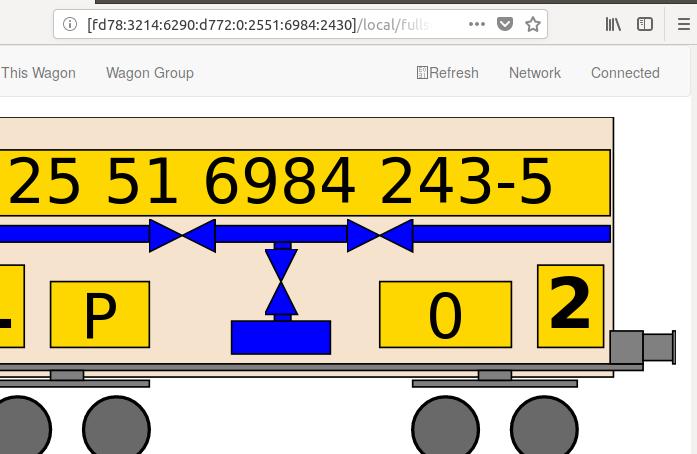
\includegraphics[width=\textwidth]{Bilder/ipv6_concept.png}
    \caption{Mögliche Darstellung des virtuellen \gls{Gueterwagen}s mit IPv6-Netzwerkadresse\cite{GAK}}
    \label{fig:IPv6}
\end{figure}
Alle Wagen sollen hierarchisch gleich gestellt sein. außerdem darf keine Abhängigkeit zu Netzwerkverbindungen oder Servern bestehen. Darum soll durch Dezentralität und lokalen Netzwerken immer eine lokale Verbindung bestehen. In dieser wird eine lokale Hierarchie gebildet.\par
Im Verband mit anderen Wagen verhält sich der \gls{Gueterwagen 40} sozial und teilt alle notwendigen Informationen über sich mit den anderen Wagen und der Lok als gleichberechtigte Partner. Dazu gehören bauartspezifische Parameter wie Gewicht, Länge, Achszahl, maximal Zuladung und Höchstgeschwindigkeit genauso wie wagenspezifische Informationen wie Besitzer, Laufleistung, Informationen aus den Sensoren, letzte Wartungen und nächste Instandhaltungszyklen.\par
Aufgrund der vielen unterschiedlich konfigurierten \gls{Gueterwagen} und Zugängen zu Daten und Akten wird eine NoSQL-Technologie als Datenbankformat gewählt. Diese sorgt auch bei unterschiedlichen Versionen und Daten für eine zukunftssichere Datenbank.\par
Eine weitere Beschreibung des Bordrechners ist in Kapitel \ref{sec:eKomp} zu finden, die Beschreibung der Kommunikation in Kapitel \ref{sec:dKomp} zu finden.

    %\section{Arbeitspaket 3 - Entwicklung Aktorik}
    \section{Konzept elektrischer Komponenten}\label{sec:eKomp}
In diesem Kapitel werden die elektrischen Komponenten innerhalb des Konstruktes \gls{Gueterwagen 40} mit ihrem Konzept einzeln beschrieben. Dieses Kapitel ist zugehörig zum Arbeitspaket 3 - Entwicklung Aktorik; genauer AP 3a: Konzeptentwicklung Aktorik und Aktorsteuerung und behandelt die elektrischen Komponenten; die pneumatischen Aktoren werden im folgenden Kapitel beschrieben.\par
Die elektrischen Komponenten sind in Abbildung \ref{fig:eKomp} farblich hervorgehoben.
Für den \gls{Demonstrator} sind drei große, elektrische Module geplant: Batterie, Bordelektronik und die Ladeelektronik, bestehend aus dem Radsatzgenerator und einer Ladeschnittstelle zur externen Aufladung (alle in blau dargestellt). Zusätzlich müssen auch alle weiteren Aktoren und Sensoren sowie Datenschnittstellen außerhalb dieser Elektronik mit Spannung versorgt werden (hier in schwarz gestrichelt dargestellt).\par
\begin{figure}[hbt]
    \centering
    \pgfdeclarelayer{background}
\pgfdeclarelayer{foreground}
\pgfdeclarelayer{Beschriftung}
%Farbendefinition
\definecolor{elek}{RGB}{55,126,184}%blau
\definecolor{pneu}{RGB}{105,105,105}%grau
\definecolor{sens}{RGB}{105,105,105}%grau
\definecolor{dat}{RGB}{105,105,105}%grau
\definecolor{strom}{RGB}{0,0,0}%schwarz

\tikzset{wagon/.style={draw = gray, ultra thick, opacity = 0.7}}
\tikzset{seite/.style={opacity = 1}}
\tikzset{elek/.style= {draw = elek, ultra thick, opacity = 1}} %elektrische Komponenten
\tikzset{sens/.style={draw = sens, ultra thick, opacity = 1}} %sensorische Komponenten
\tikzset{pneu/.style={draw = pneu, ultra thick, opacity = 1}} %pneumatische Komponenten
\tikzset{dat/.style={draw = dat, ultra thick, opacity = 1}} %Datenkomponenten
\tikzset{strom/.style={draw = strom, ultra thick, opacity = 1}} %Strom- und Datenleitungen
\tikzset{annotation/.style={draw = black, thick, opacity = 0.7, font=\scriptsize}}

\pgfsetlayers{background,main,Beschriftung,foreground}
\begin{tikzpicture}[scale=0.6]
%%%%%%%%%%%%%%%%%%%%%%%%%%%%%%%%%%%%%%%%%%%%%%%% Hintergrund %%%%%%%%%%%%%%%%%%%%%%%%%%%%%%%%%%%%%%%%%%%%%
    \begin{pgfonlayer}{background}
    %Seiten
        %Seite A
        \path[seite] (0, 3) rectangle +(.6,.2) node[pos = 0.5] (seiteA) {Seite A};
        %Seite B
        \path[seite] (0, -3.2) rectangle +(.6,.2) node[pos = 0.5] (seiteB) {Seite B};
        %Seite 1
        \path[seite] (-12.3, 0) rectangle +(.6,.2) node[pos = 0.5] (seiteB) {Seite 1};
        %Seite 2
        \path[seite] (10.3, 0) rectangle +(.6,.2) node[pos = 0.5] (seiteB) {Seite 2};      
    %wagon als Basis
    \path[wagon] (-5,-2) -- (-5,2) -- (5,2) -- (5,-2) -- cycle;
    % HL
    \path[wagon, color=pneu] (-5,-.5) -- (5,-.5) node[pos = 0.6, above] {\color=\gray \tiny{HL}};
    % Buffer
    \begin{scope}[shift = {(-5,1.5)}]
    	\path[wagon] (-.8,.3) -- (0,.3) -- (0,-.3) -- (-.8,-.3);
    	\path[wagon] (-1,.25) -- (-.8,.25) -- (-.8,-.25) -- (-1,-.25);
    	\path[wagon] (-1,-.5) .. controls (-1.05,0) and (-1.05,0) .. (-1,.5);
    \end{scope}
    \begin{scope}[shift = {(-5,-1.5)}]
    	\path[wagon] (-.8,.3) -- (0,.3) -- (0,-.3) -- (-.8,-.3);
    	\path[wagon] (-1,.25) -- (-.8,.25) -- (-.8,-.25) -- (-1,-.25);
    	\path[wagon] (-1,-.5) .. controls (-1.05,0) and (-1.05,0) .. (-1,.5);
    \end{scope}
    \begin{scope}[shift = {(5,-1.5)}, rotate = 180]
    	\path[wagon] (-.8,.3) -- (0,.3) -- (0,-.3) -- (-.8,-.3);
    	\path[wagon] (-1,.25) -- (-.8,.25) -- (-.8,-.25) -- (-1,-.25);
    	\path[wagon] (-1,-.5) .. controls (-1.05,0) and (-1.05,0) .. (-1,.5);
    \end{scope}
    \begin{scope}[shift = {(5,1.5)}, rotate = 180]
    	\path[wagon] (-.8,.3) -- (0,.3) -- (0,-.3) -- (-.8,-.3);
    	\path[wagon] (-1,.25) -- (-.8,.25) -- (-.8,-.25) -- (-1,-.25);
    	\path[wagon] (-1,-.5) .. controls (-1.05,0) and (-1.05,0) .. (-1,.5);
    \end{scope}
    %Wheelset
    \begin{scope}[shift = {(-4,0)}]
    	\path[wagon] (-.1,1.7) -- (.1,1.7) -- (.1,-1.7) -- (-.1, -1.7) -- cycle; 
    	\path[wagon] (-.6,1.4) -- (.6,1.4) -- (.55,1.5) -- (-.55, 1.5) -- cycle; 
    	\path[wagon] (-.6,-1.4) -- (.6,-1.4) -- (.55,-1.5) -- (-.55, -1.5) -- cycle; 
    \end{scope}
        \begin{scope}[shift = {(-2.5,0)}]
    	\path[wagon] (-.1,1.7) -- (.1,1.7) -- (.1,-1.7) -- (-.1, -1.7) -- cycle; 
    	\path[wagon] (-.6,1.4) -- (.6,1.4) -- (.55,1.5) -- (-.55, 1.5) -- cycle; 
    	\path[wagon] (-.6,-1.4) -- (.6,-1.4) -- (.55,-1.5) -- (-.55, -1.5) -- cycle; 
    \end{scope}
    \begin{scope}[shift = {(4,0)}]
    	\path[wagon] (-.1,1.7) -- (.1,1.7) -- (.1,-1.7) -- (-.1, -1.7) -- cycle; 
    	\path[wagon] (-.6,1.4) -- (.6,1.4) -- (.55,1.5) -- (-.55, 1.5) -- cycle; 
    	\path[wagon] (-.6,-1.4) -- (.6,-1.4) -- (.55,-1.5) -- (-.55, -1.5) -- cycle; 
    \end{scope}
    \begin{scope}[shift = {(2.5,0)}]
    	\path[wagon] (-.1,1.7) -- (.1,1.7) -- (.1,-1.7) -- (-.1, -1.7) -- cycle; 
    	\path[wagon] (-.6,1.4) -- (.6,1.4) -- (.55,1.5) -- (-.55, 1.5) -- cycle; 
    	\path[wagon] (-.6,-1.4) -- (.6,-1.4) -- (.55,-1.5) -- (-.55, -1.5) -- cycle; 
    \end{scope}
    \end{pgfonlayer}
%%%%%%%%%%%%%%%%%%%%%%%%%%%%%%%%%%%%%%%%%%%%%%% Vordergrung %%%%%%%%%%%%%%%%%%%%%%%%%%%%%%%%%%%%%%%%%%%%%%%%%
    \begin{pgfonlayer}{foreground} %Komponete
    %elektronische Komponenten
        %Radsatzgenerator
        \path[elek, fill = elek, thin] (-4.3, -1.9) rectangle +(.6,.2) node[pos = 0.5] (wsg) {};
        %Rechner
        \path[elek, fill = elek, thin] (-.5, -1.6) rectangle +(1,.3) node[pos = 0.5] (bcu) {};
        %Batterie
        \path[elek, fill = elek, thin] (-1.8, -1.8) rectangle +(1,.5) node[pos = 0.5] (bat) {};
        %optionale Ladeelektronik
        \path[elek, fill = elek, thin] (-1.8, 1.2) rectangle +(0.8,.4) node[pos = 0.5] (ole) {};
    % pneumatische Komponenten
        %epBremse
        \path[pneu, fill = pneu] (.9,-1.3) rectangle (1.1,-1.5) node[pos = 0.5] (epb) {};
        %Endabsperrhähne
        \path[pneu, fill = pneu] (-5.2, -.4) rectangle (-5,-.6) node[pos = 0.5] (eca) {};
        \path[pneu, fill = pneu] (5.2, -.4) rectangle (5,-.6) node[pos = 0.5] (ecb) {};
        %Aktorik Bremse
        \path[pneu, fill = pneu, thin] (-.5, 0) rectangle +(1,.5) node[pos = 0.5] (bcu2) {};
    %sensorische Komponenten
        %drahtloserSensor
        \path[sens, fill = sens, thin] (3.9, -1.7) rectangle +(.2,-.2) node[pos = 0.5] (wss) {};
        %Flachstellendektektor
        \path[sens, fill=sens, thin] (3.15, 1.8) rectangle +(.2,-.2) node[pos = 0.5] (flachstelle) {};
        \path[sens, fill=sens, thin] (-3.35, 1.8) rectangle +(.2,-.2) node[pos = 0.5] (flachstelle2) {};
        %Laufleistung
        \path[sens, fill = sens, thin] (3.9, 0) rectangle +(.2,-.2) node[pos = 0.5] (ll) {};
    %Datenkomponeten
        %Kurzstreckenfunk
        \path[dat, fill = dat] (-5.2, -.9) rectangle (-5,-1.05)node[pos = 0.5] (sra) {};
        \path[dat, fill = dat] (5.2, -.9) rectangle (5,-1.05)node[pos = 0.5] (srb) {};
        \path[dat, fill = dat] (5.2, .9) rectangle (5,1.05)node[pos = 0.5] (src) {};
        \path[dat, fill = dat] (-5.2, .9) rectangle (-5,1.05) node[pos = 0.5] (srd) {};
    \end{pgfonlayer}
%%%%%%%%%%%%%%%%%%%%%%%%%%%%%%%%%%%%%%%%%%%%%%% Beschriftung %%%%%%%%%%%%%%%%%%%%%%%%%%%%%%%%%%%%%%%%%%%%%%%%%
    \begin{pgfonlayer}{Beschriftung}
    %elektronische Komponenten
        %Radsatzgenerator
        \path[annotation, thin] (wsg) -- +(-.5,-.5) node[left] {Radsatzgenerator};
        %Rechner
        \path[annotation, thin] (bcu) -- +(1,-1) node[right] {Bordelektronik};
        %Batterie
        \path[annotation, thin] (bat) -- +(-1,-1) node[left] {Batterie};
        %optionale Ladeelektronik
        \path[annotation, thin] (ole) -- +(-.9,.9) node[left] {externe Ladeschnittstelle};
    %pneumatische Komponenten
        %epBremse
        \path[annotation, thin] (epb) -- +(.4,-.4) node[right] {ep-Bremse};
        %Endabsperrhähne
        \path[annotation, thin] (eca) -- +(-.5,.5) node[left] {Aktor Endabsperrhahn};
        %Aktorik Bremse
        \path[annotation, thin] (bcu2) -- +(.5,.5) node[right] {Aktorik Bremse};
    %sensorische Komponenten
        %drahtloserSensor
        \path[annotation, thin] (wss) -- +(.5,-.5) node[right] {Laufleistung}; 
        %Flachstellen
        \path[annotation, thin] (flachstelle) -- +(.7,.7) node[right] {Lagertemperatur};
        \path[annotation, thin] (flachstelle2) -- +(7.2,.7) node[right] {};
        %Laufleistung
        \path[annotation, thin] (ll) -- +(1.2,.5) node[right] {Beschleunigungen};
    %Datenkomponeten
        %Kurzstreckenfunk
        \path[annotation, thin] (srd) -- +(-.5,-.5) node[left] {Kurzstreckenfunk};    
    \end{pgfonlayer}
%%%%%%%%%%%%%%%%%%%%%%%%%%%%%%%%%%%%%%%%%%%%%% Main %%%%%%%%%%%%%%%%%%%%%%%%%%%%%%%%%%%%%%%%%%%%%%%%%%%%
    \begin{pgfonlayer}{main} %Leitungen
    %elek
        %Radsatzgenerator
        \path[elek] (wsg) +(-.1,0) -| (-3.3, -1);%-- +(1,0) -- (-3.2,-1);
        \path[strom, dashed] (wsg) +(-.1,0) -| (-3.3, -1);%-- +(1,0) -- (-3.2,-1);
        %Rechner
        \path[elek] (bcu) +(0,0)  -- (0,-1);
        \path[strom, dashed] (bcu) +(0,0)  -- (0,-1);
        %Batterie
        \path[elek] (bat) +(0,0)  -- (-1.3,-1);
        \path[strom, dashed] (bat) +(0,0)  -- (-1.3,-1);
        %optionale Ladeelektronik
        \path[elek] (ole) +(0,0)  -- (-1.35,-1);
        \path[strom, dashed] (ole) +(0,0)  -- (-1.35,-1);
    %pneu
        %ep-Bremse
        \path[pneu] (1,-.5) -- (1,-1.3);
        %\path[strom, dashed] (1,-.5) -- (1,-1.3);
        \path[pneu] (epb) +(.1,0) -- +(-.5,0);
        \path[strom, dashed] (epb) +(.1,0) -- +(-.5,0);
        %Endabsperrhähne
        \path[pneu] (eca) +(-.1,0) -- +(.2,0) -- (-4.9,-1);
        \path[strom, dashed] (eca) +(-.1,0) -- +(.2,0) -- (-4.9,-1);
        \path[pneu] (ecb) +(.1,0) -- +(-.2,0) -- (4.9,-1);
        \path[strom, dashed] (ecb) +(.1,0) -- +(-.2,0) -- (4.9,-1);
        %Aktorik Bremse
        \path[pneu] (bcu2) +(0,0)  -- (0,-1);
        \path[strom, dashed] (bcu2) +(0,0)  -- (0,-1);
    %Sensorische Kompoenten
        %Flachstellen
        \path[sens] (flachstelle)+(0,0) -- (3.2, -1);
        \path[strom, dashed] (flachstelle)+(0,0) -- (3.2, -1);
        \path[sens] (flachstelle2) +(0,0)-- (-3.3, -1);
        \path[strom, dashed] (flachstelle2) +(0,0)-- (-3.3, -1);
        %Laufleistung
        \path[sens] (ll)+(0,0) -- (4, -1);
        \path[strom, dashed] (ll)+(0,0) -- (4, -1);
        %drahloser Sensor
        \path[strom, dotted] (wss)+(0,0) -- (4, -1);
    %Strom- und Datenleitung
        \path[dat] (-5,-1) -- (5,-1);
        \path[strom, dashed] (-5,-1) -- (5,-1);
        %Kurzstreckenfunk
        \path[dat] (srd) +(-.1,0) -- +(.3,0) -- (-4.8,-1);
        \path[strom, dashed] (srd) +(-.1,0) -- +(.3,0) -- (-4.8,-1);
        \path[dat] (src) +(.1,0) -- +(-.3,0) -- (4.8,-1);
        \path[strom, dashed] (src) +(.1,0) -- +(-.3,0) -- (4.8,-1);
    \end{pgfonlayer}

\end{tikzpicture}

    \caption{elektrische Komponenten des Gesamtsystems}
    \label{fig:eKomp}
\end{figure}
Für den serienreifen \gls{Gueterwagen 40} ist auch eine Aufladung der Batterie durch eine Automatische Kupplung oder fest verlegte Kabel denkbar, diese sollen für den \gls{Demonstrator} aber noch nicht betrachtet werden.

\paragraph{Achsdeckelgenerator} \label{sec:RSG}
Das elektrische Konzept sieht vor, dass ein Radsatz- oder Achsdeckelgenerator im Umlauf des Wagens genug Energie produziert um alle notwendigen Komponenten zu speisen sowie zusätzlich eine Pufferbatterie für den geplanten und ungeplanten Fall des Stillstandes lädt.
\paragraph{Externe Ladeschnittstelle}
Zur Aufladung der \gls{Systembatterie} im Stillstand wird eine externe Ladeschnittstelle benötigt. Diese ist auch für Lokomotiven üblich und soll übernommen werden. Für die \gls{Demonstrator}en ist sie besonders wichtig, da sie keinen Üblichen Umlauf fahren.
\paragraph{Batterie}\label{sec:Batterie}
Die Batterie benötigt genügend Leistung für eine übliche Speisung der Bord- elektronik, der Aktoren und Sensoren sowie einen Puffer bei ungeplanten Zeitverzöger- ungen bei einem üblichen Wagenumlauf.
\paragraph{Bordelektronik}
Die Bordelektronik steuert alle für den \gls{Gueterwagen} notwendigen Prozesse. Dazu gehören sichere und nicht sichere Prozesse.\par
Bei sicheren Prozessen wird von außen reiner Lesezugriff gewährt. Bei nicht sicheren Funktionen ist auch ein Schreibrecht von außen zu geben. Siehe dazu auch die Systemarchitektur des Rechners im Kapitel \ref{sec:dKomp}.\par
Zu den sicheren Funktionen gehören:
\begin{itemize}
    \item Steuerung der pneumatischen und elektrischen Aktoren,
    \item Kommunikation mit den Sensoren,
    \item Speicherung der Daten der Sensoren,
    \item Steuerung und Regelung des Lademanagments,
    \item Kommunikation mit anderen \gls{Gueterwagen 40} und Lokomotiven.
\end{itemize}
Nicht sichere Funktionen dagegen können von außen im Stand und von entsprechen autorisierten Personen beschrieben werden. Zu diesen gehören:
\begin{itemize}
    \item Kommunikation mit dem Bediener
    \item Speicherung weiterer Informationen über den \gls{Gueterwagen},
    \item Kommunikation mit der Cloud zur Aktualisierung des 'Digitalen Zwillings'.
\end{itemize} %\newpage
    \section{Konzept pneumatischer Komponenten} \label{sec:pKomp}
In diesem Kapitel werden die pneumatischen Komponenten mit ihrem dahinterstehenden Konzept einzeln beschrieben. Dieses Kapitel ist zugehörig zum Arbeitspaket 3 - Entwicklung Aktorik; genauer AP 3a: Konzeptentwicklung Aktorik und Aktorsteuerung und behandelt die (pneumatischen) Aktoren.\par
Die pneumatischen Komponenten sind in Abbildung \ref{fig:pKomp} in grün farblich hervorgehoben.\par
Für den \gls{Demonstrator} ist eine teilautomatisierte Bremssteuerung geplant. Diese beinhaltet die Aktorik des Güterwagens 4.0 - siehe dazu Abbildung \ref{fig:UIC-Bremse} auf Seite \pageref{fig:UIC-Bremse} und den Anhang \ref{sec:A_Bremse40} zur \gls{Bremse 4.0} - die Aktoren an den Endabsperrhähnen und \gls{ep-assist-Bremsen}. Das Steuerventil 4.0 besteht neben dem unangetasteten UIC-Steuerventil und den unangetasteten A- und R-Kammern auch aus einigen Aktoren.\par
\begin{figure}[hbt]
    \centering
    \pgfdeclarelayer{background}
\pgfdeclarelayer{foreground}
\pgfdeclarelayer{Beschriftung}
%Farbendefinition
\definecolor{elek}{RGB}{105,105,105}%grau{55,126,184}%blau
\definecolor{pneu}{RGB}{77,175,74}%grün{pneu}{RGB}{105,105,105}%grau
\definecolor{sens}{RGB}{105,105,105}%grau
\definecolor{dat}{RGB}{105,105,105}%grau
\definecolor{strom}{RGB}{105,105,105}%grau %{0,0,0}%schwarz

\tikzset{wagon/.style={draw = gray, ultra thick, opacity = 0.7}}
\tikzset{seite/.style={opacity = 1}}
\tikzset{elek/.style= {draw = elek, ultra thick, opacity = 1}} %elektrische Komponenten
\tikzset{sens/.style={draw = sens, ultra thick, opacity = 1}} %sensorische Komponenten
\tikzset{pneu/.style={draw = pneu, ultra thick, opacity = 1}} %pneumatische Komponenten
\tikzset{dat/.style={draw = dat, ultra thick, opacity = 1}} %Datenkomponenten
\tikzset{strom/.style={draw = strom, ultra thick, opacity = 1}} %Strom- und Datenleitungen
\tikzset{annotation/.style={draw = black, thick, opacity = 0.7, font=\scriptsize}}

\pgfsetlayers{background,main,Beschriftung,foreground}
\begin{tikzpicture}[scale=0.6]
%%%%%%%%%%%%%%%%%%%%%%%%%%%%%%%%%%%%%%%%%%%%%%%% Hintergrund %%%%%%%%%%%%%%%%%%%%%%%%%%%%%%%%%%%%%%%%%%%%%
    \begin{pgfonlayer}{background}
    %Seiten
        %Seite A
        \path[seite] (0, 3) rectangle +(.6,.2) node[pos = 0.5] (seiteA) {Seite A};
        %Seite B
        \path[seite] (0, -3.2) rectangle +(.6,.2) node[pos = 0.5] (seiteB) {Seite B};
        %Seite 1
        \path[seite] (-12.3, 0) rectangle +(.6,.2) node[pos = 0.5] (seiteB) {Seite 1};
        %Seite 2
        \path[seite] (10.3, 0) rectangle +(.6,.2) node[pos = 0.5] (seiteB) {Seite 2};      
    %wagon als Basis
    \path[wagon] (-5,-2) -- (-5,2) -- (5,2) -- (5,-2) -- cycle;
    % HL
    \path[wagon, color=pneu] (-5,-.5) -- (5,-.5) node[pos = 0.6, above] {\color=\gray \tiny{HL}};
    % Buffer
    \begin{scope}[shift = {(-5,1.5)}]
    	\path[wagon] (-.8,.3) -- (0,.3) -- (0,-.3) -- (-.8,-.3);
    	\path[wagon] (-1,.25) -- (-.8,.25) -- (-.8,-.25) -- (-1,-.25);
    	\path[wagon] (-1,-.5) .. controls (-1.05,0) and (-1.05,0) .. (-1,.5);
    \end{scope}
    \begin{scope}[shift = {(-5,-1.5)}]
    	\path[wagon] (-.8,.3) -- (0,.3) -- (0,-.3) -- (-.8,-.3);
    	\path[wagon] (-1,.25) -- (-.8,.25) -- (-.8,-.25) -- (-1,-.25);
    	\path[wagon] (-1,-.5) .. controls (-1.05,0) and (-1.05,0) .. (-1,.5);
    \end{scope}
    \begin{scope}[shift = {(5,-1.5)}, rotate = 180]
    	\path[wagon] (-.8,.3) -- (0,.3) -- (0,-.3) -- (-.8,-.3);
    	\path[wagon] (-1,.25) -- (-.8,.25) -- (-.8,-.25) -- (-1,-.25);
    	\path[wagon] (-1,-.5) .. controls (-1.05,0) and (-1.05,0) .. (-1,.5);
    \end{scope}
    \begin{scope}[shift = {(5,1.5)}, rotate = 180]
    	\path[wagon] (-.8,.3) -- (0,.3) -- (0,-.3) -- (-.8,-.3);
    	\path[wagon] (-1,.25) -- (-.8,.25) -- (-.8,-.25) -- (-1,-.25);
    	\path[wagon] (-1,-.5) .. controls (-1.05,0) and (-1.05,0) .. (-1,.5);
    \end{scope}
    %Wheelset
    \begin{scope}[shift = {(-4,0)}]
    	\path[wagon] (-.1,1.7) -- (.1,1.7) -- (.1,-1.7) -- (-.1, -1.7) -- cycle; 
    	\path[wagon] (-.6,1.4) -- (.6,1.4) -- (.55,1.5) -- (-.55, 1.5) -- cycle; 
    	\path[wagon] (-.6,-1.4) -- (.6,-1.4) -- (.55,-1.5) -- (-.55, -1.5) -- cycle; 
    \end{scope}
        \begin{scope}[shift = {(-2.5,0)}]
    	\path[wagon] (-.1,1.7) -- (.1,1.7) -- (.1,-1.7) -- (-.1, -1.7) -- cycle; 
    	\path[wagon] (-.6,1.4) -- (.6,1.4) -- (.55,1.5) -- (-.55, 1.5) -- cycle; 
    	\path[wagon] (-.6,-1.4) -- (.6,-1.4) -- (.55,-1.5) -- (-.55, -1.5) -- cycle; 
    \end{scope}
    \begin{scope}[shift = {(4,0)}]
    	\path[wagon] (-.1,1.7) -- (.1,1.7) -- (.1,-1.7) -- (-.1, -1.7) -- cycle; 
    	\path[wagon] (-.6,1.4) -- (.6,1.4) -- (.55,1.5) -- (-.55, 1.5) -- cycle; 
    	\path[wagon] (-.6,-1.4) -- (.6,-1.4) -- (.55,-1.5) -- (-.55, -1.5) -- cycle; 
    \end{scope}
    \begin{scope}[shift = {(2.5,0)}]
    	\path[wagon] (-.1,1.7) -- (.1,1.7) -- (.1,-1.7) -- (-.1, -1.7) -- cycle; 
    	\path[wagon] (-.6,1.4) -- (.6,1.4) -- (.55,1.5) -- (-.55, 1.5) -- cycle; 
    	\path[wagon] (-.6,-1.4) -- (.6,-1.4) -- (.55,-1.5) -- (-.55, -1.5) -- cycle; 
    \end{scope}
    \end{pgfonlayer}
%%%%%%%%%%%%%%%%%%%%%%%%%%%%%%%%%%%%%%%%%%%%%%% Vordergrung %%%%%%%%%%%%%%%%%%%%%%%%%%%%%%%%%%%%%%%%%%%%%%%%%
    \begin{pgfonlayer}{foreground} %Komponete
    %elektronische Komponenten
        %Radsatzgenerator
        \path[elek, fill = elek, thin] (-4.3, -1.9) rectangle +(.6,.2) node[pos = 0.5] (wsg) {};
        %Rechner
        \path[elek, fill = elek, thin] (-.5, -1.6) rectangle +(1,.3) node[pos = 0.5] (bcu) {};
        %Batterie
        \path[elek, fill = elek, thin] (-1.8, -1.8) rectangle +(1,.5) node[pos = 0.5] (bat) {};
        %optionale Ladeelektronik
        \path[elek, fill = elek, thin] (-1.8, 1.2) rectangle +(0.8,.4) node[pos = 0.5] (ole) {};
    % pneumatische Komponenten
        %epBremse
        \path[pneu, fill = pneu] (.9,-1.3) rectangle (1.1,-1.5) node[pos = 0.5] (epb) {};
        %Endabsperrhähne
        \path[pneu, fill = pneu] (-5.2, -.4) rectangle (-5,-.6) node[pos = 0.5] (eca) {};
        \path[pneu, fill = pneu] (5.2, -.4) rectangle (5,-.6) node[pos = 0.5] (ecb) {};
        %Aktorik Bremse
        \path[pneu, fill = pneu, thin] (-.5, 0) rectangle +(1,.5) node[pos = 0.5] (bcu2) {};
    %sensorische Komponenten
        %drahtloserSensor
        \path[sens, fill = sens, thin] (3.9, -1.7) rectangle +(.2,-.2) node[pos = 0.5] (wss) {};
        %Flachstellendektektor
        \path[sens, fill=sens, thin] (3.15, 1.8) rectangle +(.2,-.2) node[pos = 0.5] (flachstelle) {};
        \path[sens, fill=sens, thin] (-3.35, 1.8) rectangle +(.2,-.2) node[pos = 0.5] (flachstelle2) {};
        %Laufleistung
        \path[sens, fill = sens, thin] (3.9, 0) rectangle +(.2,-.2) node[pos = 0.5] (ll) {};
    %Datenkomponeten
        %Kurzstreckenfunk
        \path[dat, fill = dat] (-5.2, -.9) rectangle (-5,-1.05)node[pos = 0.5] (sra) {};
        \path[dat, fill = dat] (5.2, -.9) rectangle (5,-1.05)node[pos = 0.5] (srb) {};
        \path[dat, fill = dat] (5.2, .9) rectangle (5,1.05)node[pos = 0.5] (src) {};
        \path[dat, fill = dat] (-5.2, .9) rectangle (-5,1.05) node[pos = 0.5] (srd) {};
    \end{pgfonlayer}
%%%%%%%%%%%%%%%%%%%%%%%%%%%%%%%%%%%%%%%%%%%%%%% Beschriftung %%%%%%%%%%%%%%%%%%%%%%%%%%%%%%%%%%%%%%%%%%%%%%%%%
    \begin{pgfonlayer}{Beschriftung}
    %elektronische Komponenten
        %Radsatzgenerator
        \path[annotation, thin] (wsg) -- +(-.5,-.5) node[left] {Radsatzgenerator};
        %Rechner
        \path[annotation, thin] (bcu) -- +(1,-1) node[right] {Bordelektronik};
        %Batterie
        \path[annotation, thin] (bat) -- +(-1,-1) node[left] {Batterie};
        %optionale Ladeelektronik
        \path[annotation, thin] (ole) -- +(-.9,.9) node[left] {externe Ladeschnittstelle};
    %pneumatische Komponenten
        %epBremse
        \path[annotation, thin] (epb) -- +(.4,-.4) node[right] {ep-Bremse};
        %Endabsperrhähne
        \path[annotation, thin] (eca) -- +(-.5,.5) node[left] {Aktor Endabsperrhahn};
        %Aktorik Bremse
        \path[annotation, thin] (bcu2) -- +(.5,.5) node[right] {Aktorik Bremse};
    %sensorische Komponenten
        %drahtloserSensor
        \path[annotation, thin] (wss) -- +(.5,-.5) node[right] {Laufleistung}; 
        %Flachstellen
        \path[annotation, thin] (flachstelle) -- +(.7,.7) node[right] {Lagertemperatur};
        \path[annotation, thin] (flachstelle2) -- +(7.2,.7) node[right] {};
        %Laufleistung
        \path[annotation, thin] (ll) -- +(1.2,.5) node[right] {Beschleunigungen};
    %Datenkomponeten
        %Kurzstreckenfunk
        \path[annotation, thin] (srd) -- +(-.5,-.5) node[left] {Kurzstreckenfunk};    
    \end{pgfonlayer}
%%%%%%%%%%%%%%%%%%%%%%%%%%%%%%%%%%%%%%%%%%%%%% Main %%%%%%%%%%%%%%%%%%%%%%%%%%%%%%%%%%%%%%%%%%%%%%%%%%%%
    \begin{pgfonlayer}{main} %Leitungen
    %elek
        %Radsatzgenerator
        \path[elek] (wsg) +(-.1,0) -| (-3.3, -1);%-- +(1,0) -- (-3.2,-1);
        \path[strom, dashed] (wsg) +(-.1,0) -| (-3.3, -1);%-- +(1,0) -- (-3.2,-1);
        %Rechner
        \path[elek] (bcu) +(0,0)  -- (0,-1);
        \path[strom, dashed] (bcu) +(0,0)  -- (0,-1);
        %Batterie
        \path[elek] (bat) +(0,0)  -- (-1.3,-1);
        \path[strom, dashed] (bat) +(0,0)  -- (-1.3,-1);
        %optionale Ladeelektronik
        \path[elek] (ole) +(0,0)  -- (-1.35,-1);
        \path[strom, dashed] (ole) +(0,0)  -- (-1.35,-1);
    %pneu
        %ep-Bremse
        \path[pneu] (1,-.5) -- (1,-1.3);
        %\path[strom, dashed] (1,-.5) -- (1,-1.3);
        \path[pneu] (epb) +(.1,0) -- +(-.5,0);
        \path[strom, dashed] (epb) +(.1,0) -- +(-.5,0);
        %Endabsperrhähne
        \path[pneu] (eca) +(-.1,0) -- +(.2,0) -- (-4.9,-1);
        \path[strom, dashed] (eca) +(-.1,0) -- +(.2,0) -- (-4.9,-1);
        \path[pneu] (ecb) +(.1,0) -- +(-.2,0) -- (4.9,-1);
        \path[strom, dashed] (ecb) +(.1,0) -- +(-.2,0) -- (4.9,-1);
        %Aktorik Bremse
        \path[pneu] (bcu2) +(0,0)  -- (0,-1);
        \path[strom, dashed] (bcu2) +(0,0)  -- (0,-1);
    %Sensorische Kompoenten
        %Flachstellen
        \path[sens] (flachstelle)+(0,0) -- (3.2, -1);
        \path[strom, dashed] (flachstelle)+(0,0) -- (3.2, -1);
        \path[sens] (flachstelle2) +(0,0)-- (-3.3, -1);
        \path[strom, dashed] (flachstelle2) +(0,0)-- (-3.3, -1);
        %Laufleistung
        \path[sens] (ll)+(0,0) -- (4, -1);
        \path[strom, dashed] (ll)+(0,0) -- (4, -1);
        %drahloser Sensor
        \path[strom, dotted] (wss)+(0,0) -- (4, -1);
    %Strom- und Datenleitung
        \path[dat] (-5,-1) -- (5,-1);
        \path[strom, dashed] (-5,-1) -- (5,-1);
        %Kurzstreckenfunk
        \path[dat] (srd) +(-.1,0) -- +(.3,0) -- (-4.8,-1);
        \path[strom, dashed] (srd) +(-.1,0) -- +(.3,0) -- (-4.8,-1);
        \path[dat] (src) +(.1,0) -- +(-.3,0) -- (4.8,-1);
        \path[strom, dashed] (src) +(.1,0) -- +(-.3,0) -- (4.8,-1);
    \end{pgfonlayer}

\end{tikzpicture}

    \caption{Pneumatische Komponenten des Gesamtsystems}
    \label{fig:pKomp}
\end{figure}
Alle Aktoren, abgesehen von denen für \gls{ep-assist-Bremsen}, sollen, zur Gewährleistung von gleicher Sicherheit, vor Fahrtantritt abschaltbar sein. Damit sie in der geforderten Position bleiben werden bistabile Magnetventile und Stellmotoren verwendet. Diese halten sicher ihre Stellung auch ohne Stromversorgung. So ist nur darüber ein Nachweis zu führen.\par
Die \gls{Bremse 4.0} besteht aus der Hauptluftleitung, dem Bremsgestänge, dem Steuerventil 4.0, einem Relaisventil, zwei C-Druck-Sensoren, der Feststellbremse und \gls{ep-assist-Bremsen}.\par
\begin{figure}
    \centering%[hbt]
    %\includegraphics[width=10cm%\textwidth
    %]{Bilder/Abb3_Druckluftbremse.png}
    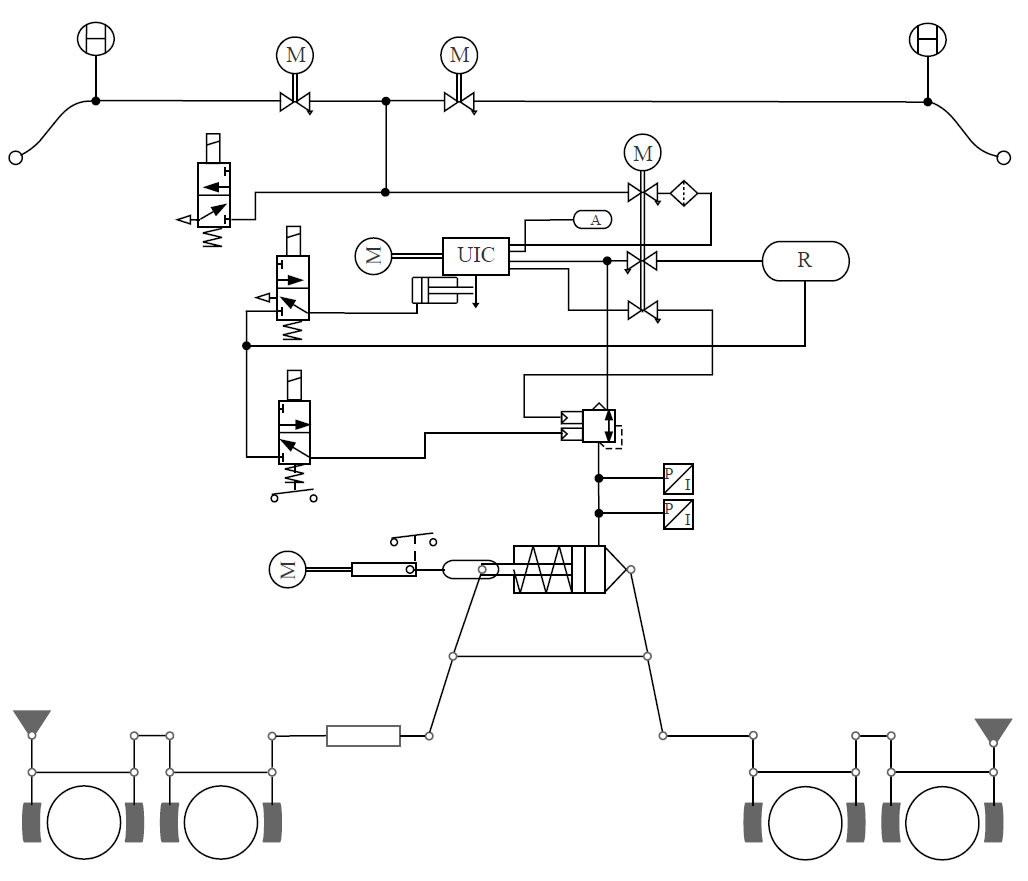
\includegraphics[width=10cm]{Bilder/GW40Schema.PNG}
    \caption{UIC-kompatible Druckluftbremse des Güterwagen 4.0}% \cite{ETR_2}}
    \label{fig:UIC-Bremse}
\end{figure}
\paragraph{Hauptluftleitung} Die \gls{HL} besteht aus der \gls{HL} selbst, den Endabsperrhähnen, die bei der \gls{Bremse 4.0} als Muffenkugelhahn ausgeführt werden, zwei Schauzeichen für den Druck der \gls{HL} und der üblichen Schlauchkupplung.

\paragraph{Endabsperrhahn} \label{sec:Endabsperrhahn}
An beiden Enden des Wagens werden die Endabsperrhähne mit zu- sätzliche Ventilen ausgestattet. Diese sorgen für eine sichere Trennung und Kupplung von Wagen durch automatisches öffnen und schließen. Zusätzlich bieten sie eine wichtige Unterstützung zur automatischen \gls{Bremsprobe}, da sie direkt ansteuerbar sind. Sie sind mit passender Zustandsanzeige auszustatten.

\paragraph{Bremsgestänge} Das Bremsgestänge bleibt wie gewohnt. Einzig der \gls{Lastwechsel} wird ausgebaut und im Relaisventil (s.u.) automatisiert. Ebenso bleibt der Verschleißnachsteller.

\paragraph{Steuerventil}\label{sec:Bremsart}
Das Steuerventil 4.0 besteht aus einem UIC/\acrshort{TSI}-kompatiblen Steuerventil mit A-Kammer, einer G/P-Umstellvorrichtung mit visueller Zustandsanzeige, Schnell- lösen und Bremse aus. Für die Funktion Bremse aus wird auch eine visuelle Zustandsanzeige benötigt.

\paragraph{Relaisventil} Das Relaisventil wird für die automatische Lastabbremsung verwendet. Dazu besitzt es ein Vorsteuerventil mit Rückmeldeschalter. Zur besseren Übersicht wird auch hier eine visuelle Zustandsanzeigeüber die \gls{Lastwechsel}stellung benötigt.

\paragraph{C-Druck-Sensor} \label{sec:C-Druck}
Der C-Druck (Bremszylinderdruck) wird zwischen Relaisventil und Bremszylinder gemessen und für die \gls{Bremsprobe} benötigt. Es werden zwei Sensoren mit unabhängiger Messung verwendet. Dies ermöglicht eine Zweikanaligkeit für diesen Messwert.

\paragraph{Feststellbremse} Die Feststellbremse besteht aus einem Stellmotor mit mechanischer Übersetzung, einem Rückmeldeschalter und einer visuellen Zustandsanzeige. Durch die Einführung der automatischen Feststellbremse fällt das Legen von \gls{Hemmschuh}en vor dem Wagen weg.

\paragraph{ep-Assist} Bei  \gls{ep-assist-Bremsen} wird die \gls{HL} lokal entlüftet. Ein ep-Lösen findet nicht statt\footnote{Dafür würde eine Hauptbehälterluftleitung benötigt werden, diese ist im Allgemeinen bei \gls{Gueterwagen} nicht vorhanden, darum kann und soll diese Funktion nicht umgesetzt werden. Die indirekte Bremsfunktion bleibt vorhanden.}.  Die elektrische Ansteuerung sorgt für kürzere Durchschlagzeiten, für weniger Verschleiß durch weniger auffahren und kürzere Bremswege durch schnelle Bremsanspruchzeiten. Dafür wird ein weiteres pneumatisches Zwei-Wege-Ventil benötigt.

\paragraph{Zustandsanzeige pneumatische Aktoren}\label{sec:ZustandKupplung}
Die pneumatische Bremse benötigt aufgrund der veränderten Technik diverse Zustandsanzeigen. Diese sind sämtlich elektro-mecha- nisch oder elektro-pneumatisch ausgeführt, damit sie auch eine sichere Anzeige bieten, wenn das System vor der \gls{Zugfahrt} abgeschaltet wird.\par
Folgende Zustandsanzeigen sind vorgesehen:
\begin{itemize}
    \item Druckanzeige der Schlauchkupplung
    \item Zustand G/P-Umsteller
    \item Zustand Bremse (eingeschaltet / ausgeschaltet)
    \item Zustand \gls{Lastwechsel}
    \item Zustand Feststellbremse
\end{itemize}
%Aktor der zweikanalig den Zustand der pneumatischen Hähne (drucklos, druckbeaufschlagt) anzeigt.
 %\newpage
    \section{Konzept sensorischer Komponenten}
In diesem Kapitel werden die sensorischen Komponenten des \gls{Gueterwagen 40} einzeln beschrieben. Dieses Kapitel ist zugehörig zum Arbeitspaket 4 - Entwicklung Sensorik; genauer AP 4a: Konzeptentwicklung Sensorik und behandelt den sensorischen Teil des \gls{Gueterwagen 40} inklusive Condition Monitoring.\par
Die sensorischen Komponenten sind in Abbildung \ref{fig:sKomp} in rot farblich aufgezeigt.
\begin{figure}[hbt]
    \centering
    \pgfdeclarelayer{background}
\pgfdeclarelayer{foreground}
\pgfdeclarelayer{Beschriftung}
%Farbendefinition
\definecolor{elek}{RGB}{105,105,105}%grau{55,126,184}%blau
\definecolor{pneu}{RGB}{105,105,105}%grau
\definecolor{sens}{RGB}{228,26,28}%rot{105,105,105}%grau
\definecolor{dat}{RGB}{105,105,105}%grau
\definecolor{strom}{RGB}{105,105,105}%grau %{0,0,0}%schwarz

\tikzset{wagon/.style={draw = gray, ultra thick, opacity = 0.7}}
\tikzset{seite/.style={opacity = 1}}
\tikzset{elek/.style= {draw = elek, ultra thick, opacity = 1}} %elektrische Komponenten
\tikzset{sens/.style={draw = sens, ultra thick, opacity = 1}} %sensorische Komponenten
\tikzset{pneu/.style={draw = pneu, ultra thick, opacity = 1}} %pneumatische Komponenten
\tikzset{dat/.style={draw = dat, ultra thick, opacity = 1}} %Datenkomponenten
\tikzset{strom/.style={draw = strom, ultra thick, opacity = 1}} %Strom- und Datenleitungen
\tikzset{annotation/.style={draw = black, thick, opacity = 0.7, font=\scriptsize}}

\pgfsetlayers{background,main,Beschriftung,foreground}
\begin{tikzpicture}[scale=0.6]
%%%%%%%%%%%%%%%%%%%%%%%%%%%%%%%%%%%%%%%%%%%%%%%% Hintergrund %%%%%%%%%%%%%%%%%%%%%%%%%%%%%%%%%%%%%%%%%%%%%
    \begin{pgfonlayer}{background}
    %Seiten
        %Seite A
        \path[seite] (0, 3) rectangle +(.6,.2) node[pos = 0.5] (seiteA) {Seite A};
        %Seite B
        \path[seite] (0, -3.2) rectangle +(.6,.2) node[pos = 0.5] (seiteB) {Seite B};
        %Seite 1
        \path[seite] (-12.3, 0) rectangle +(.6,.2) node[pos = 0.5] (seiteB) {Seite 1};
        %Seite 2
        \path[seite] (10.3, 0) rectangle +(.6,.2) node[pos = 0.5] (seiteB) {Seite 2};      
    %wagon als Basis
    \path[wagon] (-5,-2) -- (-5,2) -- (5,2) -- (5,-2) -- cycle;
    % HL
    \path[wagon, color=pneu] (-5,-.5) -- (5,-.5) node[pos = 0.6, above] {\color=\gray \tiny{HL}};
    % Buffer
    \begin{scope}[shift = {(-5,1.5)}]
    	\path[wagon] (-.8,.3) -- (0,.3) -- (0,-.3) -- (-.8,-.3);
    	\path[wagon] (-1,.25) -- (-.8,.25) -- (-.8,-.25) -- (-1,-.25);
    	\path[wagon] (-1,-.5) .. controls (-1.05,0) and (-1.05,0) .. (-1,.5);
    \end{scope}
    \begin{scope}[shift = {(-5,-1.5)}]
    	\path[wagon] (-.8,.3) -- (0,.3) -- (0,-.3) -- (-.8,-.3);
    	\path[wagon] (-1,.25) -- (-.8,.25) -- (-.8,-.25) -- (-1,-.25);
    	\path[wagon] (-1,-.5) .. controls (-1.05,0) and (-1.05,0) .. (-1,.5);
    \end{scope}
    \begin{scope}[shift = {(5,-1.5)}, rotate = 180]
    	\path[wagon] (-.8,.3) -- (0,.3) -- (0,-.3) -- (-.8,-.3);
    	\path[wagon] (-1,.25) -- (-.8,.25) -- (-.8,-.25) -- (-1,-.25);
    	\path[wagon] (-1,-.5) .. controls (-1.05,0) and (-1.05,0) .. (-1,.5);
    \end{scope}
    \begin{scope}[shift = {(5,1.5)}, rotate = 180]
    	\path[wagon] (-.8,.3) -- (0,.3) -- (0,-.3) -- (-.8,-.3);
    	\path[wagon] (-1,.25) -- (-.8,.25) -- (-.8,-.25) -- (-1,-.25);
    	\path[wagon] (-1,-.5) .. controls (-1.05,0) and (-1.05,0) .. (-1,.5);
    \end{scope}
    %Wheelset
    \begin{scope}[shift = {(-4,0)}]
    	\path[wagon] (-.1,1.7) -- (.1,1.7) -- (.1,-1.7) -- (-.1, -1.7) -- cycle; 
    	\path[wagon] (-.6,1.4) -- (.6,1.4) -- (.55,1.5) -- (-.55, 1.5) -- cycle; 
    	\path[wagon] (-.6,-1.4) -- (.6,-1.4) -- (.55,-1.5) -- (-.55, -1.5) -- cycle; 
    \end{scope}
        \begin{scope}[shift = {(-2.5,0)}]
    	\path[wagon] (-.1,1.7) -- (.1,1.7) -- (.1,-1.7) -- (-.1, -1.7) -- cycle; 
    	\path[wagon] (-.6,1.4) -- (.6,1.4) -- (.55,1.5) -- (-.55, 1.5) -- cycle; 
    	\path[wagon] (-.6,-1.4) -- (.6,-1.4) -- (.55,-1.5) -- (-.55, -1.5) -- cycle; 
    \end{scope}
    \begin{scope}[shift = {(4,0)}]
    	\path[wagon] (-.1,1.7) -- (.1,1.7) -- (.1,-1.7) -- (-.1, -1.7) -- cycle; 
    	\path[wagon] (-.6,1.4) -- (.6,1.4) -- (.55,1.5) -- (-.55, 1.5) -- cycle; 
    	\path[wagon] (-.6,-1.4) -- (.6,-1.4) -- (.55,-1.5) -- (-.55, -1.5) -- cycle; 
    \end{scope}
    \begin{scope}[shift = {(2.5,0)}]
    	\path[wagon] (-.1,1.7) -- (.1,1.7) -- (.1,-1.7) -- (-.1, -1.7) -- cycle; 
    	\path[wagon] (-.6,1.4) -- (.6,1.4) -- (.55,1.5) -- (-.55, 1.5) -- cycle; 
    	\path[wagon] (-.6,-1.4) -- (.6,-1.4) -- (.55,-1.5) -- (-.55, -1.5) -- cycle; 
    \end{scope}
    \end{pgfonlayer}
%%%%%%%%%%%%%%%%%%%%%%%%%%%%%%%%%%%%%%%%%%%%%%% Vordergrung %%%%%%%%%%%%%%%%%%%%%%%%%%%%%%%%%%%%%%%%%%%%%%%%%
    \begin{pgfonlayer}{foreground} %Komponete
    %elektronische Komponenten
        %Radsatzgenerator
        \path[elek, fill = elek, thin] (-4.3, -1.9) rectangle +(.6,.2) node[pos = 0.5] (wsg) {};
        %Rechner
        \path[elek, fill = elek, thin] (-.5, -1.6) rectangle +(1,.3) node[pos = 0.5] (bcu) {};
        %Batterie
        \path[elek, fill = elek, thin] (-1.8, -1.8) rectangle +(1,.5) node[pos = 0.5] (bat) {};
        %optionale Ladeelektronik
        \path[elek, fill = elek, thin] (-1.8, 1.2) rectangle +(0.8,.4) node[pos = 0.5] (ole) {};
    % pneumatische Komponenten
        %epBremse
        \path[pneu, fill = pneu] (.9,-1.3) rectangle (1.1,-1.5) node[pos = 0.5] (epb) {};
        %Endabsperrhähne
        \path[pneu, fill = pneu] (-5.2, -.4) rectangle (-5,-.6) node[pos = 0.5] (eca) {};
        \path[pneu, fill = pneu] (5.2, -.4) rectangle (5,-.6) node[pos = 0.5] (ecb) {};
        %Aktorik Bremse
        \path[pneu, fill = pneu, thin] (-.5, 0) rectangle +(1,.5) node[pos = 0.5] (bcu2) {};
    %sensorische Komponenten
        %drahtloserSensor
        \path[sens, fill = sens, thin] (3.9, -1.7) rectangle +(.2,-.2) node[pos = 0.5] (wss) {};
        %Flachstellendektektor
        \path[sens, fill=sens, thin] (3.15, 1.8) rectangle +(.2,-.2) node[pos = 0.5] (flachstelle) {};
        \path[sens, fill=sens, thin] (-3.35, 1.8) rectangle +(.2,-.2) node[pos = 0.5] (flachstelle2) {};
        %Laufleistung
        \path[sens, fill = sens, thin] (3.9, 0) rectangle +(.2,-.2) node[pos = 0.5] (ll) {};
    %Datenkomponeten
        %Kurzstreckenfunk
        \path[dat, fill = dat] (-5.2, -.9) rectangle (-5,-1.05)node[pos = 0.5] (sra) {};
        \path[dat, fill = dat] (5.2, -.9) rectangle (5,-1.05)node[pos = 0.5] (srb) {};
        \path[dat, fill = dat] (5.2, .9) rectangle (5,1.05)node[pos = 0.5] (src) {};
        \path[dat, fill = dat] (-5.2, .9) rectangle (-5,1.05) node[pos = 0.5] (srd) {};
    \end{pgfonlayer}
%%%%%%%%%%%%%%%%%%%%%%%%%%%%%%%%%%%%%%%%%%%%%%% Beschriftung %%%%%%%%%%%%%%%%%%%%%%%%%%%%%%%%%%%%%%%%%%%%%%%%%
    \begin{pgfonlayer}{Beschriftung}
    %elektronische Komponenten
        %Radsatzgenerator
        \path[annotation, thin] (wsg) -- +(-.5,-.5) node[left] {Radsatzgenerator};
        %Rechner
        \path[annotation, thin] (bcu) -- +(1,-1) node[right] {Bordelektronik};
        %Batterie
        \path[annotation, thin] (bat) -- +(-1,-1) node[left] {Batterie};
        %optionale Ladeelektronik
        \path[annotation, thin] (ole) -- +(-.9,.9) node[left] {externe Ladeschnittstelle};
    %pneumatische Komponenten
        %epBremse
        \path[annotation, thin] (epb) -- +(.4,-.4) node[right] {ep-Bremse};
        %Endabsperrhähne
        \path[annotation, thin] (eca) -- +(-.5,.5) node[left] {Aktor Endabsperrhahn};
        %Aktorik Bremse
        \path[annotation, thin] (bcu2) -- +(.5,.5) node[right] {Aktorik Bremse};
    %sensorische Komponenten
        %drahtloserSensor
        \path[annotation, thin] (wss) -- +(.5,-.5) node[right] {Laufleistung}; 
        %Flachstellen
        \path[annotation, thin] (flachstelle) -- +(.7,.7) node[right] {Lagertemperatur};
        \path[annotation, thin] (flachstelle2) -- +(7.2,.7) node[right] {};
        %Laufleistung
        \path[annotation, thin] (ll) -- +(1.2,.5) node[right] {Beschleunigungen};
    %Datenkomponeten
        %Kurzstreckenfunk
        \path[annotation, thin] (srd) -- +(-.5,-.5) node[left] {Kurzstreckenfunk};    
    \end{pgfonlayer}
%%%%%%%%%%%%%%%%%%%%%%%%%%%%%%%%%%%%%%%%%%%%%% Main %%%%%%%%%%%%%%%%%%%%%%%%%%%%%%%%%%%%%%%%%%%%%%%%%%%%
    \begin{pgfonlayer}{main} %Leitungen
    %elek
        %Radsatzgenerator
        \path[elek] (wsg) +(-.1,0) -| (-3.3, -1);%-- +(1,0) -- (-3.2,-1);
        \path[strom, dashed] (wsg) +(-.1,0) -| (-3.3, -1);%-- +(1,0) -- (-3.2,-1);
        %Rechner
        \path[elek] (bcu) +(0,0)  -- (0,-1);
        \path[strom, dashed] (bcu) +(0,0)  -- (0,-1);
        %Batterie
        \path[elek] (bat) +(0,0)  -- (-1.3,-1);
        \path[strom, dashed] (bat) +(0,0)  -- (-1.3,-1);
        %optionale Ladeelektronik
        \path[elek] (ole) +(0,0)  -- (-1.35,-1);
        \path[strom, dashed] (ole) +(0,0)  -- (-1.35,-1);
    %pneu
        %ep-Bremse
        \path[pneu] (1,-.5) -- (1,-1.3);
        %\path[strom, dashed] (1,-.5) -- (1,-1.3);
        \path[pneu] (epb) +(.1,0) -- +(-.5,0);
        \path[strom, dashed] (epb) +(.1,0) -- +(-.5,0);
        %Endabsperrhähne
        \path[pneu] (eca) +(-.1,0) -- +(.2,0) -- (-4.9,-1);
        \path[strom, dashed] (eca) +(-.1,0) -- +(.2,0) -- (-4.9,-1);
        \path[pneu] (ecb) +(.1,0) -- +(-.2,0) -- (4.9,-1);
        \path[strom, dashed] (ecb) +(.1,0) -- +(-.2,0) -- (4.9,-1);
        %Aktorik Bremse
        \path[pneu] (bcu2) +(0,0)  -- (0,-1);
        \path[strom, dashed] (bcu2) +(0,0)  -- (0,-1);
    %Sensorische Kompoenten
        %Flachstellen
        \path[sens] (flachstelle)+(0,0) -- (3.2, -1);
        \path[strom, dashed] (flachstelle)+(0,0) -- (3.2, -1);
        \path[sens] (flachstelle2) +(0,0)-- (-3.3, -1);
        \path[strom, dashed] (flachstelle2) +(0,0)-- (-3.3, -1);
        %Laufleistung
        \path[sens] (ll)+(0,0) -- (4, -1);
        \path[strom, dashed] (ll)+(0,0) -- (4, -1);
        %drahloser Sensor
        \path[strom, dotted] (wss)+(0,0) -- (4, -1);
    %Strom- und Datenleitung
        \path[dat] (-5,-1) -- (5,-1);
        \path[strom, dashed] (-5,-1) -- (5,-1);
        %Kurzstreckenfunk
        \path[dat] (srd) +(-.1,0) -- +(.3,0) -- (-4.8,-1);
        \path[strom, dashed] (srd) +(-.1,0) -- +(.3,0) -- (-4.8,-1);
        \path[dat] (src) +(.1,0) -- +(-.3,0) -- (4.8,-1);
        \path[strom, dashed] (src) +(.1,0) -- +(-.3,0) -- (4.8,-1);
    \end{pgfonlayer}

\end{tikzpicture}

    \caption{Sensorische Komponenten des Gesamtsystems}
    \label{fig:sKomp}
\end{figure}
Für den \gls{Demonstrator} ist eine Teilausstattung mit Sensoren geplant. Diese dienen zum Auslesen von Aktoren sowie zur Zustandsüberwachung des Wagens.\par
Folgende Zustände von \gls{40-Komponenten} sollen überwacht werden:
\begin{itemize}
    \item Batteriestand
    \item Pneumatische Kupplung
    \item Steuerventilstellung
    \item Relaisventilstellung
    \item Stellung der \gls{HL}-Ventile
    \item Stellung der Feststellbremse
    \item C-Druck
\end{itemize}
Zusätzlich soll auch der Zustand des Wagens überwacht werden. Dafür sind folgende Sensoren vorgesehen:
\begin{itemize}
    \item Lagertemperatur
    \item Beschleunigungen in x-, y- und z-Richtung
    \item Laufleistung/Radumdrehung
    %\item Flachstellendetektion an jedem Rad
    %\item Lagertemperatur an jedem Lager
    %\item Geschwindigkeit an jeder Achse
    %\item Laufleistung an jeder Achse
    %\item Stoßsensor an jeder Wagenseite
    %\item Bremsbelagüberwachung an jeder Bremszange
\end{itemize}

\begin{comment}
\subsection{Konzept}
Condition Monitoring\\
Laderaumtemperatur\\
Türüberwachung\\
Stöße\\
Flachstellendetektion\\
Geschwindikeit\\
Laufleistung\\
Bremsbelag\\
Temperaturen\\
Batteriestand
\end{comment}
 %\newpage
    \section{Konzept Datenkommunikation}\label{sec:dKomp}
In diesem Kapitel geht es um die konzeptuelle Ausführung der Datenkommunikation. Es teilt sich auf in die Teile Hardware und Software und ist zugehörig zum Arbeitspaket 5 - Datenkommunikation; genauer AP 5a: Entwicklung eines Hardware- und Software-Konzepts für die Kommunikation und behandelt die Ausführung der notwendigen Daten und deren Kommunikationsmöglichkeiten in Hard- und Software.  Auch die Rechnerarchitektur wird hier beschrieben.\par
Die entsprechenden Hardwarekomponenten sind in Abbildung \ref{fig:dKomp} in violett farblich markiert.
\begin{figure}[hbt]
    \centering
    \pgfdeclarelayer{background}
\pgfdeclarelayer{foreground}
\pgfdeclarelayer{Beschriftung}
%Farbendefinition
\definecolor{elek}{RGB}{105,105,105}%grau{55,126,184}%blau
\definecolor{pneu}{RGB}{105,105,105}%grau{77,175,74}%grün
\definecolor{sens}{RGB}{105,105,105}%grau{228,26,28}%rot
\definecolor{dat}{RGB}{152,78,163}%violett
\definecolor{strom}{RGB}{105,105,105}%grau{0,0,0}%schwarz

\tikzset{wagon/.style={draw = gray, ultra thick, opacity = 0.7}}
\tikzset{seite/.style={opacity = 1}}
\tikzset{elek/.style= {draw = elek, ultra thick, opacity = 1}} %elektrische Komponenten
\tikzset{sens/.style={draw = sens, ultra thick, opacity = 1}} %sensorische Komponenten
\tikzset{pneu/.style={draw = pneu, ultra thick, opacity = 1}} %pneumatische Komponenten
\tikzset{dat/.style={draw = dat, ultra thick, opacity = 1}} %Datenkomponenten
\tikzset{strom/.style={draw = strom, ultra thick, opacity = 1}} %Strom- und Datenleitungen
\tikzset{annotation/.style={draw = black, thick, opacity = 0.7, font=\scriptsize}}

\pgfsetlayers{background,main,Beschriftung,foreground}
\begin{tikzpicture}[scale=0.6]
%%%%%%%%%%%%%%%%%%%%%%%%%%%%%%%%%%%%%%%%%%%%%%%% Hintergrund %%%%%%%%%%%%%%%%%%%%%%%%%%%%%%%%%%%%%%%%%%%%%
    \begin{pgfonlayer}{background}
    %Seiten
        %Seite A
        \path[seite] (0, 3) rectangle +(.6,.2) node[pos = 0.5] (seiteA) {Seite A};
        %Seite B
        \path[seite] (0, -3.2) rectangle +(.6,.2) node[pos = 0.5] (seiteB) {Seite B};
        %Seite 1
        \path[seite] (-12.3, 0) rectangle +(.6,.2) node[pos = 0.5] (seiteB) {Seite 1};
        %Seite 2
        \path[seite] (10.3, 0) rectangle +(.6,.2) node[pos = 0.5] (seiteB) {Seite 2};        
        
    %wagon als Basis
    \path[wagon] (-5,-2) -- (-5,2) -- (5,2) -- (5,-2) -- cycle;
    % HL
    \path[wagon, color=pneu] (-5,-.5) -- (5,-.5) node[pos = 0.6, above] {\color=\gray \tiny{HL}};
    % Buffer
    \begin{scope}[shift = {(-5,1.5)}]
    	\path[wagon] (-.8,.3) -- (0,.3) -- (0,-.3) -- (-.8,-.3);
    	\path[wagon] (-1,.25) -- (-.8,.25) -- (-.8,-.25) -- (-1,-.25);
    	\path[wagon] (-1,-.5) .. controls (-1.05,0) and (-1.05,0) .. (-1,.5);
    \end{scope}
    \begin{scope}[shift = {(-5,-1.5)}]
    	\path[wagon] (-.8,.3) -- (0,.3) -- (0,-.3) -- (-.8,-.3);
    	\path[wagon] (-1,.25) -- (-.8,.25) -- (-.8,-.25) -- (-1,-.25);
    	\path[wagon] (-1,-.5) .. controls (-1.05,0) and (-1.05,0) .. (-1,.5);
    \end{scope}
    \begin{scope}[shift = {(5,-1.5)}, rotate = 180]
    	\path[wagon] (-.8,.3) -- (0,.3) -- (0,-.3) -- (-.8,-.3);
    	\path[wagon] (-1,.25) -- (-.8,.25) -- (-.8,-.25) -- (-1,-.25);
    	\path[wagon] (-1,-.5) .. controls (-1.05,0) and (-1.05,0) .. (-1,.5);
    \end{scope}
    \begin{scope}[shift = {(5,1.5)}, rotate = 180]
    	\path[wagon] (-.8,.3) -- (0,.3) -- (0,-.3) -- (-.8,-.3);
    	\path[wagon] (-1,.25) -- (-.8,.25) -- (-.8,-.25) -- (-1,-.25);
    	\path[wagon] (-1,-.5) .. controls (-1.05,0) and (-1.05,0) .. (-1,.5);
    \end{scope}
    %Wheelset
    \begin{scope}[shift = {(-4,0)}]
    	\path[wagon] (-.1,1.7) -- (.1,1.7) -- (.1,-1.7) -- (-.1, -1.7) -- cycle; 
    	\path[wagon] (-.6,1.4) -- (.6,1.4) -- (.55,1.5) -- (-.55, 1.5) -- cycle; 
    	\path[wagon] (-.6,-1.4) -- (.6,-1.4) -- (.55,-1.5) -- (-.55, -1.5) -- cycle; 
    \end{scope}
        \begin{scope}[shift = {(-2.5,0)}]
    	\path[wagon] (-.1,1.7) -- (.1,1.7) -- (.1,-1.7) -- (-.1, -1.7) -- cycle; 
    	\path[wagon] (-.6,1.4) -- (.6,1.4) -- (.55,1.5) -- (-.55, 1.5) -- cycle; 
    	\path[wagon] (-.6,-1.4) -- (.6,-1.4) -- (.55,-1.5) -- (-.55, -1.5) -- cycle; 
    \end{scope}
    \begin{scope}[shift = {(4,0)}]
    	\path[wagon] (-.1,1.7) -- (.1,1.7) -- (.1,-1.7) -- (-.1, -1.7) -- cycle; 
    	\path[wagon] (-.6,1.4) -- (.6,1.4) -- (.55,1.5) -- (-.55, 1.5) -- cycle; 
    	\path[wagon] (-.6,-1.4) -- (.6,-1.4) -- (.55,-1.5) -- (-.55, -1.5) -- cycle; 
    \end{scope}
    \begin{scope}[shift = {(2.5,0)}]
    	\path[wagon] (-.1,1.7) -- (.1,1.7) -- (.1,-1.7) -- (-.1, -1.7) -- cycle; 
    	\path[wagon] (-.6,1.4) -- (.6,1.4) -- (.55,1.5) -- (-.55, 1.5) -- cycle; 
    	\path[wagon] (-.6,-1.4) -- (.6,-1.4) -- (.55,-1.5) -- (-.55, -1.5) -- cycle; 
    \end{scope}
    \end{pgfonlayer}
%%%%%%%%%%%%%%%%%%%%%%%%%%%%%%%%%%%%%%%%%%%%%%% Vordergrung %%%%%%%%%%%%%%%%%%%%%%%%%%%%%%%%%%%%%%%%%%%%%%%%%
    \begin{pgfonlayer}{foreground} %Komponete
    %elektronische Komponenten
        %Radsatzgenerator
        \path[elek, fill = elek, thin] (-4.3, -1.9) rectangle +(.6,.2) node[pos = 0.5] (wsg) {};
        %Rechner
        \path[elek, fill = elek, thin] (-.5, -1.6) rectangle +(1,.3) node[pos = 0.5] (bcu) {};
        %Batterie
        \path[elek, fill = elek, thin] (-1.8, -1.8) rectangle +(1,.5) node[pos = 0.5] (bat) {};
        %optionale Ladeelektronik
        \path[elek, fill = elek, thin] (-1.8, 1.2) rectangle +(0.8,.4) node[pos = 0.5] (ole) {};
    % pneumatische Komponenten
        %epBremse
        \path[pneu, fill = pneu] (.9,-1.3) rectangle (1.1,-1.5) node[pos = 0.5] (epb) {};
        %Endabsperrhähne
        \path[pneu, fill = pneu] (-5.2, -.4) rectangle (-5,-.6) node[pos = 0.5] (eca) {};
        \path[pneu, fill = pneu] (5.2, -.4) rectangle (5,-.6) node[pos = 0.5] (ecb) {};
        %Aktorik Bremse
        \path[pneu, fill = pneu, thin] (-.5, 0) rectangle +(1,.5) node[pos = 0.5] (bcu2) {};
    %sensorische Komponenten
        %drahtloserSensor
        \path[sens, fill = sens, thin] (3.9, -1.7) rectangle +(.2,-.2) node[pos = 0.5] (wss) {};
        %Flachstellendektektor
        \path[sens, fill=sens, thin] (3.15, 1.8) rectangle +(.2,-.2) node[pos = 0.5] (flachstelle) {};
        \path[sens, fill=sens, thin] (-3.35, 1.8) rectangle +(.2,-.2) node[pos = 0.5] (flachstelle2) {};
        %Laufleistung
        \path[sens, fill = sens, thin] (3.9, 0) rectangle +(.2,-.2) node[pos = 0.5] (ll) {};
    %Datenkomponeten
        %Kurzstreckenfunk
        \path[dat, fill = dat] (-5.2, -.9) rectangle (-5,-1.05)node[pos = 0.5] (sra) {};
        \path[dat, fill = dat] (5.2, -.9) rectangle (5,-1.05)node[pos = 0.5] (srb) {};
        \path[dat, fill = dat] (5.2, .9) rectangle (5,1.05)node[pos = 0.5] (src) {};
        \path[dat, fill = dat] (-5.2, .9) rectangle (-5,1.05) node[pos = 0.5] (srd) {};
    \end{pgfonlayer}
%%%%%%%%%%%%%%%%%%%%%%%%%%%%%%%%%%%%%%%%%%%%%%% Beschriftung %%%%%%%%%%%%%%%%%%%%%%%%%%%%%%%%%%%%%%%%%%%%%%%%%
    \begin{pgfonlayer}{Beschriftung}
    %elektronische Komponenten
        %Radsatzgenerator
        \path[annotation, thin] (wsg) -- +(-.5,-.5) node[left] {Achsdeckelgenerator};
        %Rechner
        \path[annotation, thin] (bcu) -- +(1,-1) node[right] {Bordelektronik};
        %Batterie
        \path[annotation, thin] (bat) -- +(-1,-1) node[left] {Batterie};
        %optionale Ladeelektronik
        \path[annotation, thin] (ole) -- +(-.9,.9) node[left] {externe Ladeschnittstelle};
    %pneumatische Komponenten
        %epBremse
        \path[annotation, thin] (epb) -- +(.4,-.4) node[right] {ep-Bremse};
        %Endabsperrhähne
        \path[annotation, thin] (eca) -- +(-.5,.5) node[left] {Aktor Endabsperrhahn};
        %Aktorik Bremse
        \path[annotation, thin] (bcu2) -- +(.5,.5) node[right] {Aktorik Bremse};
    %sensorische Komponenten
        %drahtloserSensor
        \path[annotation, thin] (wss) -- +(.5,-.5) node[right] {Laufleistung}; 
        %Flachstellen
        \path[annotation, thin] (flachstelle) -- +(.7,.7) node[right] {Lagertemperatur};
        \path[annotation, thin] (flachstelle2) -- +(7.2,.7) node[right] {};
        %Laufleistung
        \path[annotation, thin] (ll) -- +(1.2,.5) node[right] {Beschleunigungen};
    %Datenkomponeten
        %Kurzstreckenfunk
        \path[annotation, thin] (srd) -- +(-.5,-.5) node[left] {Kurzstreckenfunk};    
    \end{pgfonlayer}
%%%%%%%%%%%%%%%%%%%%%%%%%%%%%%%%%%%%%%%%%%%%%% Main %%%%%%%%%%%%%%%%%%%%%%%%%%%%%%%%%%%%%%%%%%%%%%%%%%%%
    \begin{pgfonlayer}{main} %Leitungen
    %elek
        %Radsatzgenerator
        \path[elek] (wsg) +(-.1,0) -| (-3.3, -1);%-- +(1,0) -- (-3.2,-1);
        \path[strom, dashed] (wsg) +(-.1,0) -| (-3.3, -1);%-- +(1,0) -- (-3.2,-1);
        %Rechner
        \path[elek] (bcu) +(0,0)  -- (0,-1);
        \path[strom, dashed] (bcu) +(0,0)  -- (0,-1);
        %Batterie
        \path[elek] (bat) +(0,0)  -- (-1.3,-1);
        \path[strom, dashed] (bat) +(0,0)  -- (-1.3,-1);
        %optionale Ladeelektronik
        \path[elek] (ole) +(0,0)  -- (-1.35,-1);
        \path[strom, dashed] (ole) +(0,0)  -- (-1.35,-1);
    %pneu
        %ep-Bremse
        \path[pneu] (1,-.5) -- (1,-1.3);
        %\path[strom, dashed] (1,-.5) -- (1,-1.3);
        \path[pneu] (epb) +(.1,0) -- +(-.5,0);
        \path[strom, dashed] (epb) +(.1,0) -- +(-.5,0);
        %Endabsperrhähne
        \path[pneu] (eca) +(-.1,0) -- +(.2,0) -- (-4.9,-1);
        \path[strom, dashed] (eca) +(-.1,0) -- +(.2,0) -- (-4.9,-1);
        \path[pneu] (ecb) +(.1,0) -- +(-.2,0) -- (4.9,-1);
        \path[strom, dashed] (ecb) +(.1,0) -- +(-.2,0) -- (4.9,-1);
        %Aktorik Bremse
        \path[pneu] (bcu2) +(0,0)  -- (0,-1);
        \path[strom, dashed] (bcu2) +(0,0)  -- (0,-1);
    %Sensorische Kompoenten
        %Flachstellen
        \path[sens] (flachstelle)+(0,0) -- (3.2, -1);
        \path[strom, dashed] (flachstelle)+(0,0) -- (3.2, -1);
        \path[sens] (flachstelle2) +(0,0)-- (-3.3, -1);
        \path[strom, dashed] (flachstelle2) +(0,0)-- (-3.3, -1);
        %Laufleistung
        \path[sens] (ll)+(0,0) -- (4, -1);
        \path[strom, dashed] (ll)+(0,0) -- (4, -1);
        %drahloser Sensor
        \path[strom, dotted] (wss)+(0,0) -- (4, -1);
    %Strom- und Datenleitung
        \path[dat] (-5,-1) -- (5,-1);
        \path[strom, dashed] (-5,-1) -- (5,-1);
        %Kurzstreckenfunk
        \path[dat] (srd) +(-.1,0) -- +(.3,0) -- (-4.8,-1);
        \path[strom, dashed] (srd) +(-.1,0) -- +(.3,0) -- (-4.8,-1);
        \path[dat] (src) +(.1,0) -- +(-.3,0) -- (4.8,-1);
        \path[strom, dashed] (src) +(.1,0) -- +(-.3,0) -- (4.8,-1);
    \end{pgfonlayer}

\end{tikzpicture}

    \caption{Hardwarekomponenten zur Datenkommunikation des Gesamtsystems}
    \label{fig:dKomp}
\end{figure}
Damit die Wagen untereinander sozial interagieren können, ist eine Kommunikation untereinander ebenso notwendig wie Informationen über sich selbst. Zur Verarbeitung und Sicherung eigener Daten werden Sensoren und Aktoren ausgelesen und im Digitalen Zwilling gespeichert.\par
Dieser Digitale Zwlling wird bei der Kommunikation mit anderen Wagen, der Lok oder mobilen Device je nach Autorisierung mit Lese- oder Lese- und Schreibzugriff ausgetauscht.\par
Der Wagen besitzt, siehe Abbildung \ref{fig:Wagenkomm}, zwei, an den Längsseiten angebrachte, Möglich- keiten für den Kurzstreckenfunk zur Kommunikation mit Nachbarwagen, sowie zwei WLAN-Antennen mit eigener CPU an zwei gegenüberliegenden Ecken als Kommunikationsschnittstelle zum Bediener sowie zur Überbrückung nicht ausgerüsteter Wagen im \gls{Wagenzug}. Zusätzlich hat jeder Wagen zur Ortung und Zeitsynchronisation eine GPS-Antenne und - je nach Ausstattung - eine optionale Möglichkeit für den Fernfunk mittels GSM, GSMR, UMTS oö zum Übersenden von Daten in die Cloud. Die Kommunikation mit Sensoren und Aktoren läuft direkt über den Hauptrechner. Dieser ist leistungsstärker und beinhaltet neben der Verarbeitung der Sensor- und Aktordaten auch das Batteriemanagementsystem, sowie die Digitale Identität.\par
\begin{figure}[hbt]
    \centering
    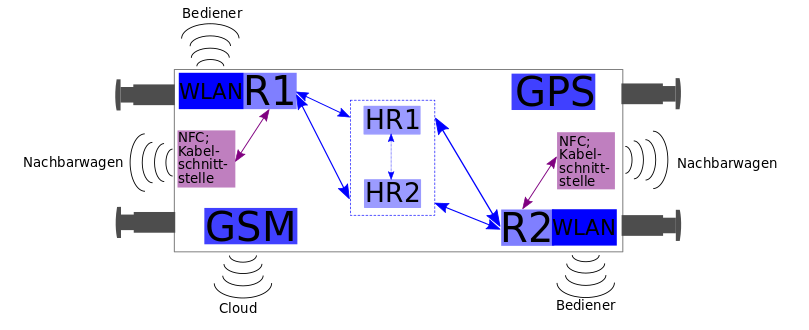
\includegraphics[width=\textwidth]{Bilder/wagen_draufsicht.png}
    \caption{Kommunikationsmöglichkeiten und angedeutete Rechnerstruktur eines einzelnen Güterwagen 4.0}
    \label{fig:Wagenkomm}
\end{figure}
Die Kommunikation im Wagen findet über ein Bussystem mit geringem spezifischen Energiebedarf statt. Für erste Tests ist EtherCAT angedacht.\par
Die Kommunikation der Wagen untereinander findet entweder, bei nicht vollständig ausgerüsteten Wagenzügen, über ein WLAN-Mesh (siehe Abbildung \ref{fig:Wagenkomm}, blau) in mittlerer Distanz oder direkt über eine Kurzdistanz-Verbindung (lila) statt. Diese Kurzdistanzverbindungen können kabelgebunden über Ethernet, NFC, WLAN mit 60GHz oder BlueTooth entstehen. Eine sinnvolle Auswahl wird im Projekt getroffen. Bei beiden Kommunikationswegen ist wichtig, dass diese sicher und unempfindlich gegenüber Störungen und Manipulation ist. Sie soll außerdem über Kurz- und Mittelstreckenfunk redundant ausgeführt sein, was zu einer  höheren Sicherheit und Zuverlässigkeit führt. Siehe dazu auch Abbildung \ref{fig:Zugkomm}. \par
Zusätzlich soll auch noch eine optionale Verbindung zu einer Cloud im Fernbereichsfunk zur Verfügung stehen. Diese erhält allerdings nur einen Lesezugriff um eine Manipulation über die Cloud so schwierig wie möglich zu gestalten.\par
\begin{figure}[hbt]
    \centering
    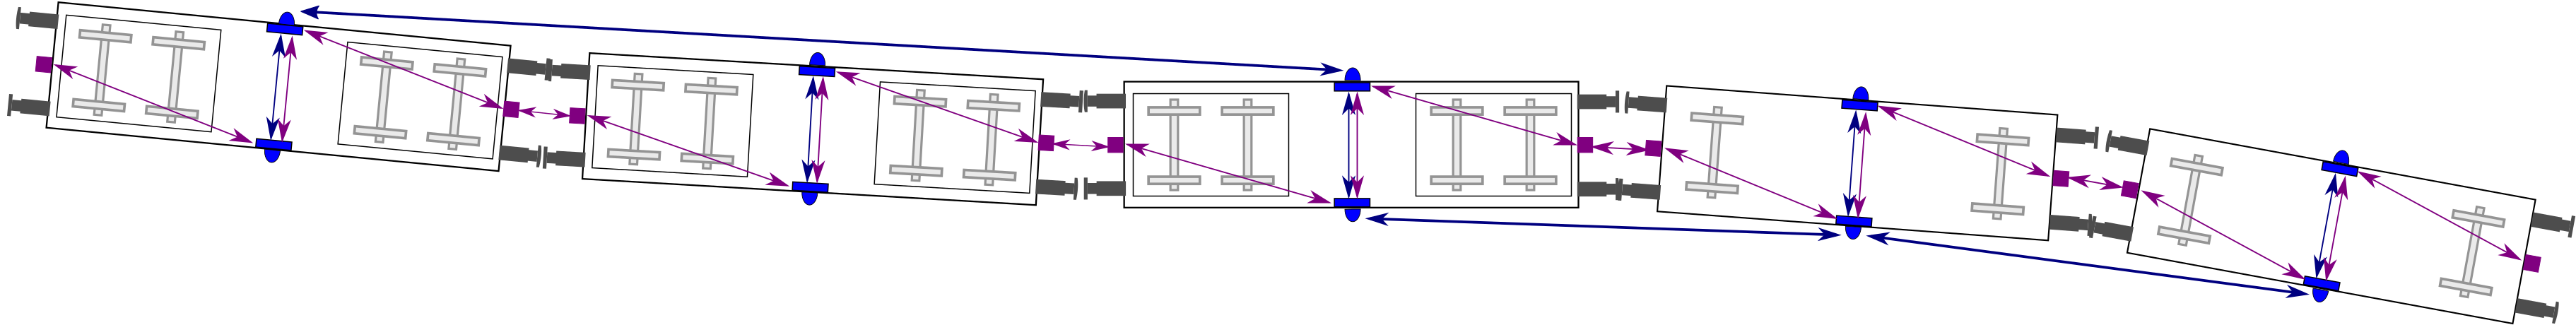
\includegraphics[width=\textwidth]{Bilder/zug_draufsicht_bogen.png}
    %\includesvg[width=\textwidth]{Bilder/zug_draufsicht_bogen}
    \caption{Kommunikation im Zugverband\cite{autonBetrieb}}
    \label{fig:Zugkomm}
\end{figure}
Die Kommunikation mit dem Bediener erfolgt lokal innerhalb des wageneigenen WLANs, bzw. des \gls{Wagenzug}es eigenen WLAN-Meshs. Eine genaue Ausarbeitung dieser Kommunikation erfolgt im Projekt. Möglich wären beipielsweise einzelne Bedienelemente mittels RFID oder QR-Code anzuwählen und am mobilen Endgerät zu bedienen.\par
Bei einer Vollausrüstung von Wagen mit Kommunikation von Wagen zu Wagen über Funk und innerhalb der Wagen über EtherCAT ist diese Kommunikation kaum störbar. Hier bietet der \gls{Gueterwagen} auch volles Potential für Zugautomatisierungen inklusive Zugtaufe, \gls{Bremsprobe} und \gls{ep-Bremsen}n. Sogar ETCS Level 3 kann möglich sein.\par
Aber auch bei nur einer Teilausrüstung der Wagen kann eine Nutzentfaltung durch Digitalisierung von Prozessen an der Ladestelle stattfinden. Eine Automatisierung ist dann in Verbindung mit stationärer Technik im Betrieb möglich.\par
Die Vernetzung zur Lok kann mittels eines Dongles an der UIC 556-Schnittstelle über das Wire-Train-Bus-Gateway stattfinden. Dies ist als Idee angedacht, wird aber nicht im Projekt umgesetzt.\par

\paragraph{Rechnerstruktur}
Damit eine sichere Datenhaltung und -übertragung möglich ist, wird die in Abbildung \ref{fig:Wagenkomm} gezeigte Rechnerarchitektur für den Hauptrechner vorgeschlagen. Diese ist eine Überlegung, muss aber noch nicht für das Labormuster oder den Demonstrator aufgebaut werden.\par
Der in der Mitte gezeigte Hauptrechner besteht aus zwei getrennten Kernen. Diese sorgen für eine Zweikanaligkeit im sicherheitskritischen Bereich. Ebenfalls zweikanalig ausgeführt ist, wie oben beschrieben, die Kommunikation mit den anderen Wagen.\par
Angedeutet sind der Bediener, dessen Schnittstelle der Nahbereichsfunk darstellt, das GSM-Modul, die Schnittstelle zur Cloud und die Sensoren, Aktoren und Kommunikationseinheiten im Wagen.\par
Die beiden Kerne im Hauptrechner tauschen sich gegenseitig rückkopplungsfrei aus und geben ihre Befehle zweikanalig an Sensoren, Aktoren und die Kommunikationseinheiten im Wagen weiter. Die zurückkommenden Informationen (rote Pfeile zu Rechner 1 und Rechner 2) werden von den Rechnern verarbeitet und im Speicher gesichert.\par
Befehle aus der Nahbereichsschnittstelle werden vom Bediener gegeben und nach Autorisierung verarbeitet. \par

\paragraph{Softwarestruktur}
Die Softwarestruktur, siehe das Diagramm in Abbildung \ref{fig:SWStruktur}, zeigt den Hauptrechner HR sowie die beiden Kommunikationsmodule R1 und R2 im \gls{Gueterwagen 40}. Angenzend dazu sind andere Wagen und ein Bediener angedeutet.
Alle Rechner sind mit einem Linuxsystem auszustatten. Zu erkennen ist, dass die beiden Kommunikationsrechner nur Schnittstellen zum Hauptrechner und zur Kommunikation mit weiteren Wagen sowie zum Bediener haben. Der Hauptrechner dagegen ist leistungsstärker und verarbeitet alle hereinkommenden Daten. Dazu gehört das BMS, die Digitale Identität, alle Sensor- und Aktordaten. Ebenso wird hier die Zugzusammenstellung und Zugtaufe ebenso wie der virtuelle Bremszettel verarbeitet. Er bietet die Intelligenz des Güterwagens 4.0.\par
Die Software selbst soll vorallem intern arbeiten und über generische Netzwerkschnittstellen kommunizieren. So kann ein häufiges verändern der Software durch Änderungen in der Hardware vermieden werden. Die Kommunikation mit der Hardware kann dann beispielsweise über eine REST-Schnittstelle erfolgen.

\begin{figure}
    \centering
    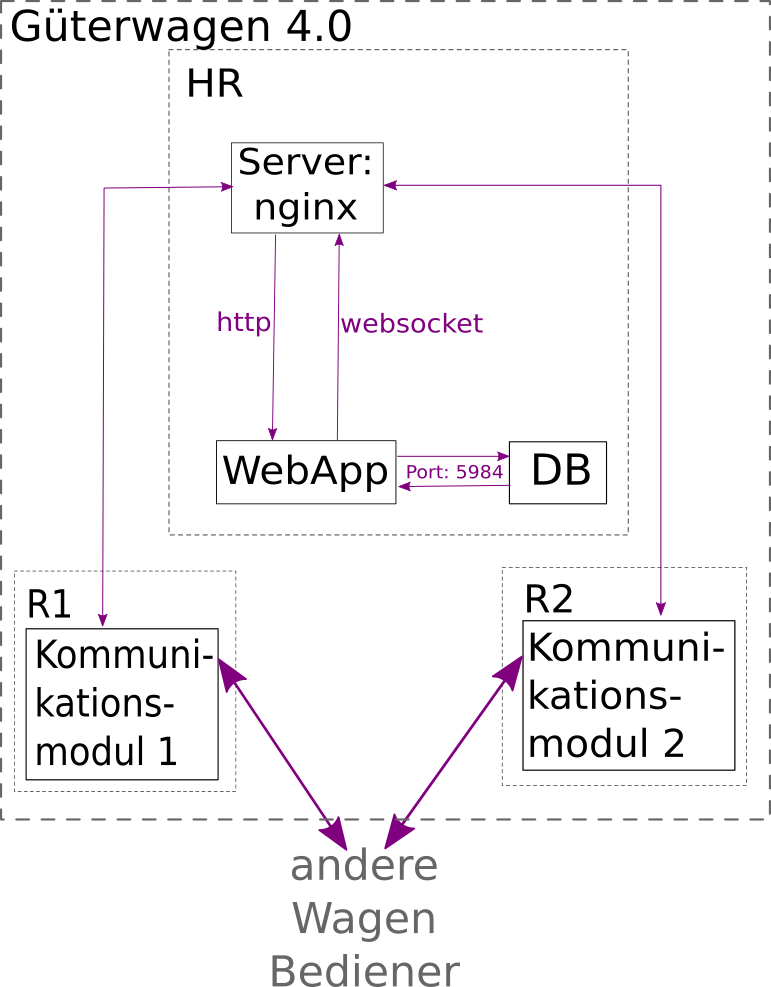
\includegraphics[width=10cm%\textwidth
    ]{Bilder/Softwarestruktur.png}
    \caption{Softwarestrukturdiagramm des Güterwagen 4.0}
    \label{fig:SWStruktur}
\end{figure}


\begin{comment}
\subsubsection{Hardware}
An Hardwarekomponenten sind Funkstellen für die Wagenkommunikation geplant.
\begin{itemize}
    \item Komponenten für Kurzstreckenfunk -- WLAN 60GHz/2,4GHz -- Wagen-Wagen, Wagen-Lok -- 1b
    \item Komponenten für mittlere Distanzen -- Wagen...Wagen, Wagen-Device
    \item Komponenten für Fernbereichsfunk -- Wagen-Cloud
\end{itemize}
\subsubsection{Software}
\begin{itemize}
    \item Lademanagement \label{sec:Lademanagment} -- 3d
    \item Anforderungen an sicheres funkgestütztes Bedienen und beobachten bei der Zugbildung -- 1d
    \item DI -- 1c
    \item \gls{WagonOS}
    \item Kommunikationsprotokolle - Datenkommunikation -- 1c
    \item automatische Zugbildung -- 1c
    \item automatische Bremsprobe -- 1c
    \item automatische Bremseinstellung
\end{itemize}
\end{comment}
 %\newpage
    %\section{Fazit} \newpage
%Hauptteil Ende

%Anhang Beginn
\pagenumbering{Roman}
    \printbibliography[heading=bibintoc, title={Quellenverzeichnis}] \newpage
    \appendix
    \section{Bremse 4.0}\label{sec:A_Bremse40}
Das vollständige Druckluftschema der \gls{Bremse 4.0}, bereits beschrieben in Kapitel \ref{sec:pKomp}, ist auf der nächsten Seite  zu sehen. Die Komponenten dazu lassen sich in Tabelle \ref{tab:Bremse40Komp} finden.
\begin{table}[h]
    \centering
    \begin{tabular}{|p{3em}cp{10.5em}p{18.5em}|}
    \hline
    Pos.  & \multicolumn{1}{p{2.5em}}{Anzahl} & Bezeichung & Zeichung / Kommentar  \\\hline
    02.01 & 2     & Aussenanzeige gls{HL} & Vergleichbar mit C-Druck-Anzeige \\
    02.02 & 2     & Endabsperrhahn 1,25" & z.B. Muffenkugelhahn Heco, Rückmeldekontakte \\
    
    04.01 & 1     & \gls{ep-Bremsen}n & Mg-Ventil NC \\
    04.02 & 1     & Kombinationsventil Bremse aus & Mechanisch gekuppelte Kugehähne, ein Antrieb, Rückmeldekontakte \\
    04.03 & 1     & Steuerventil & z.B SW4 mit G/P-Umstellung \\
    04.04 & 1     & Umstellantrieb G/P & Stellantrieb, Rückmeldekontakte \\
    04.05 & 1     & Vorsteuervenitl Schnelllösen & Mg-Ventil NC \\
    04.06 & 1     & Umstellventil Lastabbremsung & Kugelhahn 1/4", Rückmeldekontakte \\
    04.07 & 1     & Relaisventil & z.B. Faiveley VCAV \\
    04.08 & 2     & C-Druck-Sensor & 0-5 bar, 4...20 mA \\
    
    14.01 & 1     & Antrieb Feststellbremse & tbd, z.B. von PJM \\
    14.02 & 2     & Außenanzeige G/P & Mechanisch, Konstruktionsteil \\
    14.03 & 2     & Außenanzeige Leer/Beladen & Mechanisch, Konstruktionsteil \\
    14.04 & 2     & Außenanzeige Bremse aus & Mechanisch, Konstruktionsteil \\
    14.05 & 2     & Außenanzeige Feststellbremse & Mechanisch, Konstruktionsteil, 3 Zustände \\\hline
    \end{tabular}%
    \caption{Stückliste zum Druckluftschema der Bremse 4.0}
    \label{tab:Bremse40Komp}
\end{table}
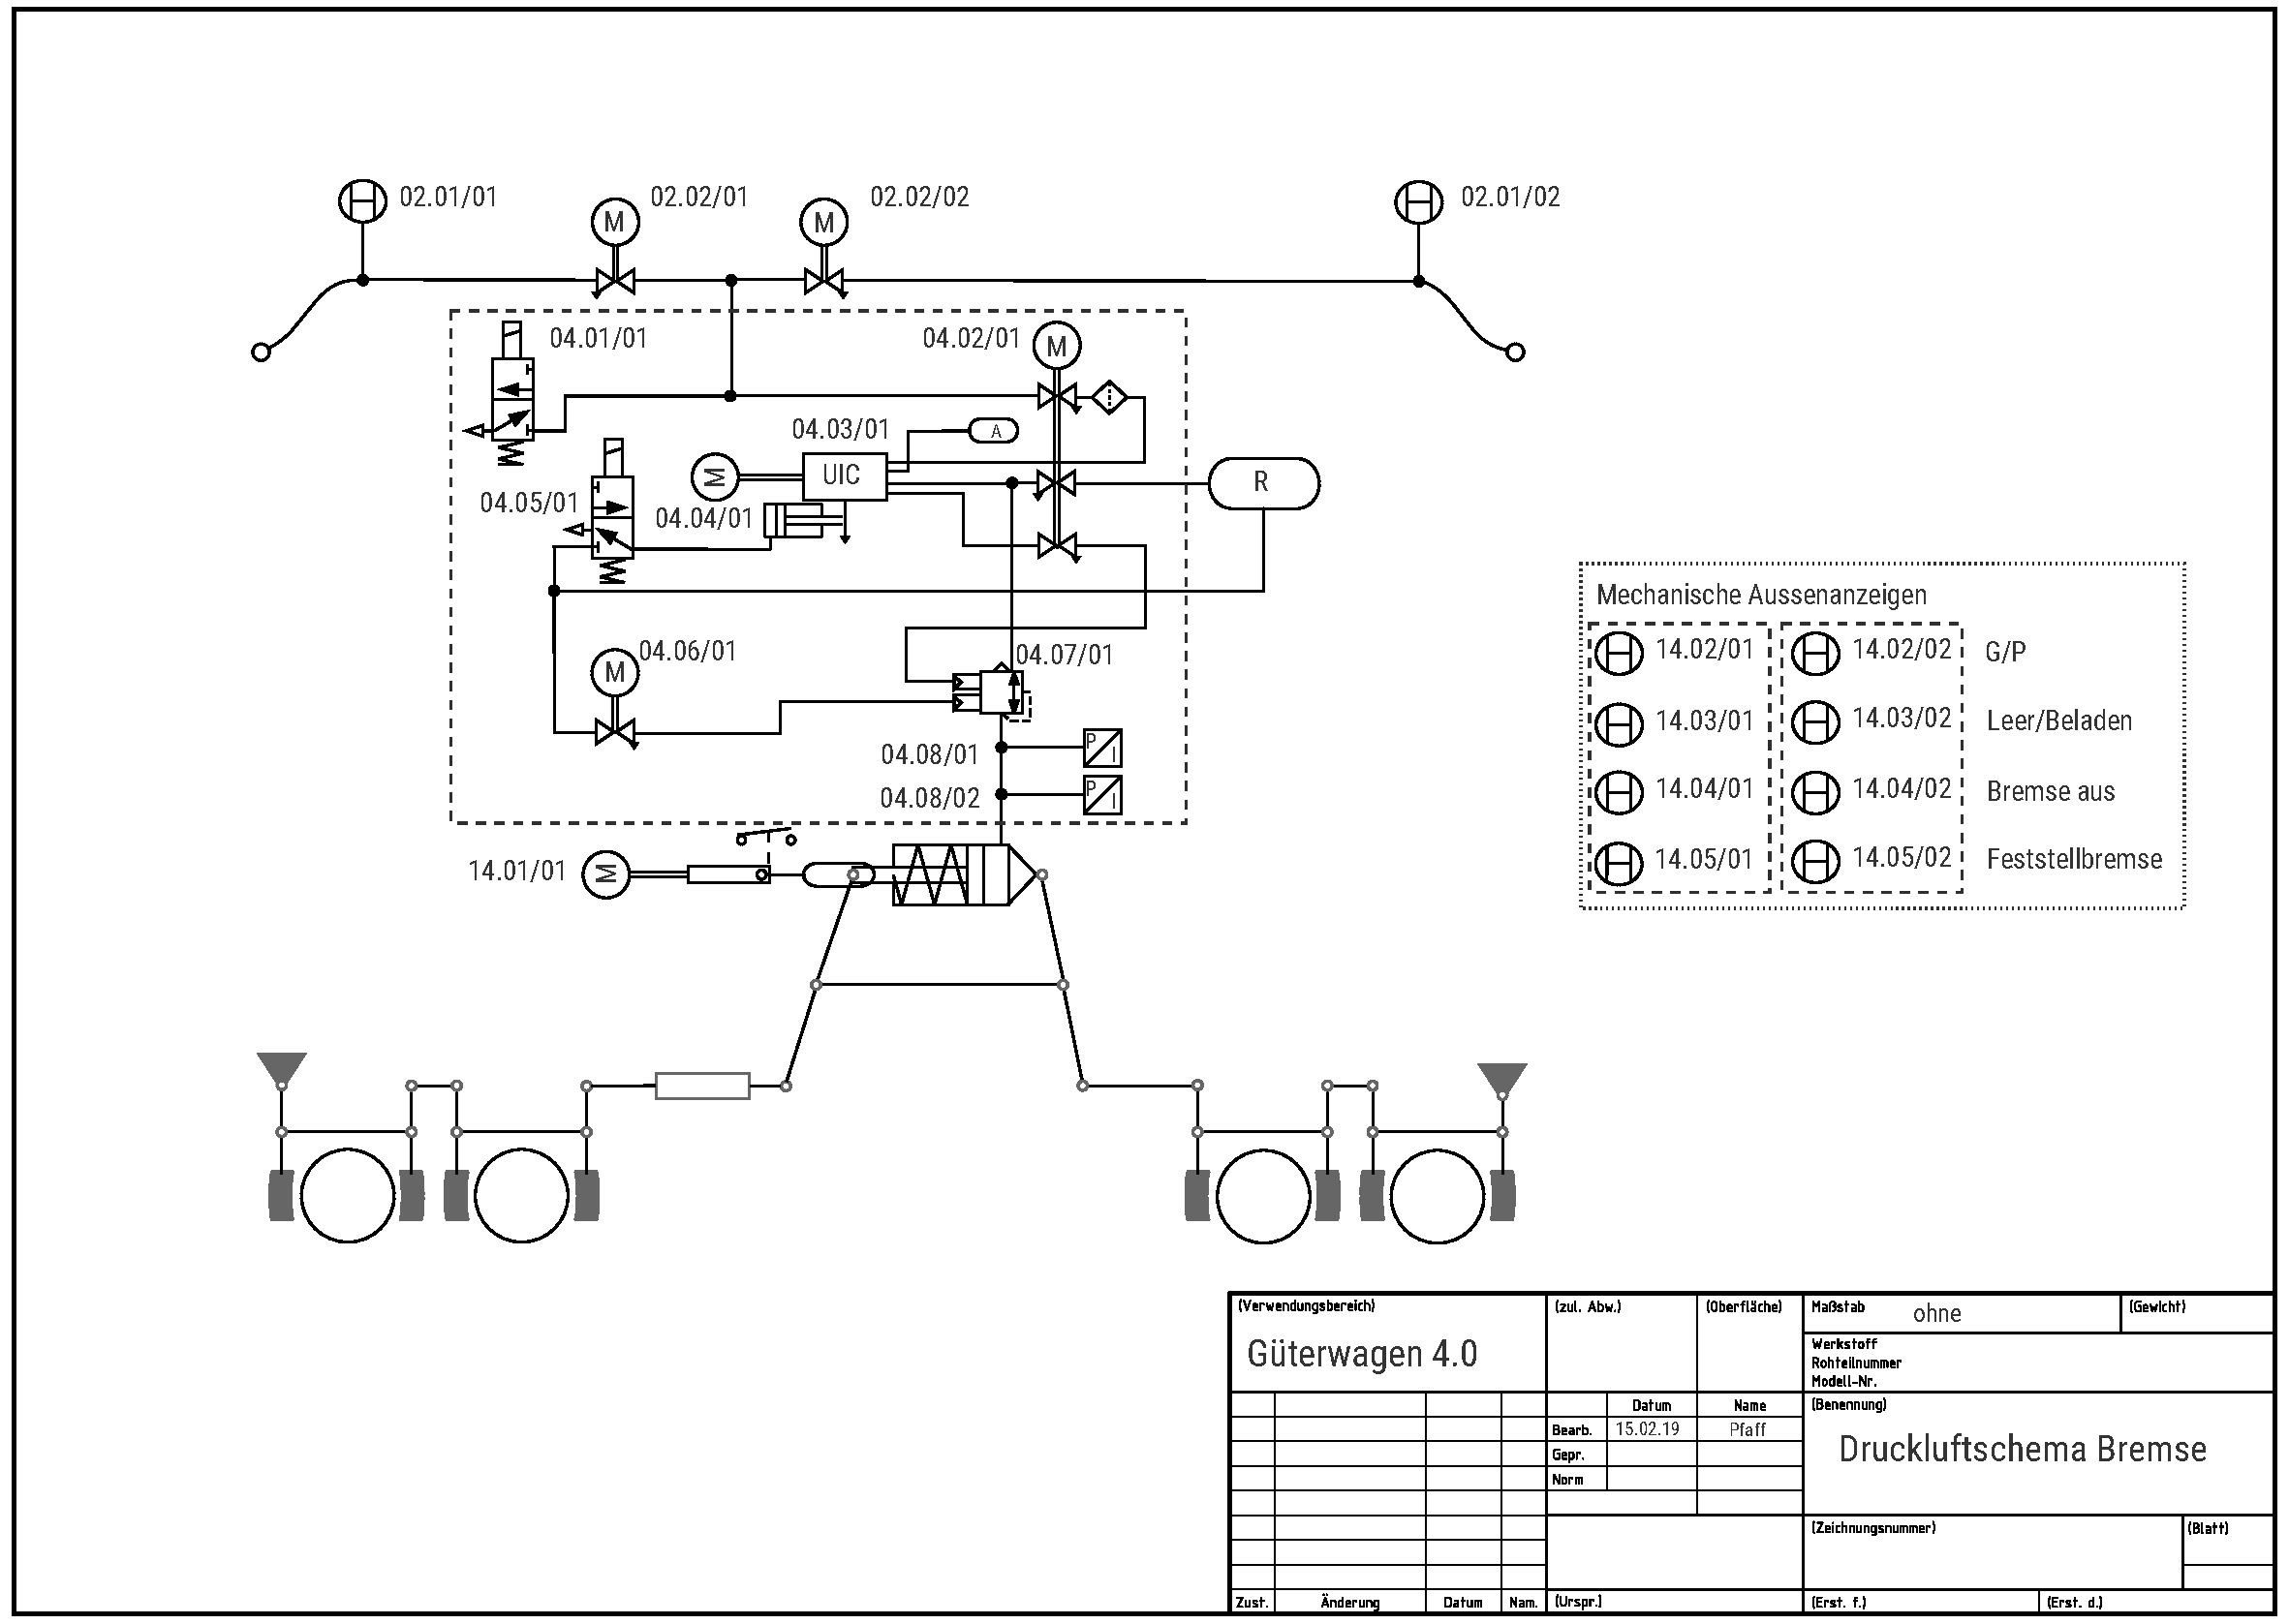
\includepdf[landscape=true, pages=-]{Bilder/PneumaticScheme.pdf}
    %\input{Kapitel/Dokumente.tex}\newpage
    %\subsection{Realisierung elektrischer Komponenten}\label{sec:eKomp}
In diesem Kapitel werden die elektrischen Komponenten einzeln beschrieben. Dieses Kapitel ist zugehörig zum Arbeitspaket 3 - Entwicklung Aktorik; genauer AP 3a: Konzeptentwicklung Aktorik und Aktorsteuerung und behandelt den die elektrischen Komponenten; die pneumatischen Aktoren werden im folgenden Kapitel beschrieben.\par
Die elektrischen Komponenten sind in Abbildung \ref{fig:eKomp} farblich hervorgehoben.
Für den Demonstrator sind drei große, elektrische Module geplant: Batterie, Bordelektronik und die Ladeelektronik, bestehend aus dem Radsatzgenerator und einer Ladeschnittstelle zur externen Aufladung (alle in blau dargestellt). Zusätzlich müssen auch alle weiteren Aktoren und Sensoren sowie Datenschnittstellen außerhalb dieser Elektronik mit Spannung versorgt werden (hier in schwarz gestrichelt dargestellt).\par
\begin{figure}[hbt]
    \centering
    \pgfdeclarelayer{background}
\pgfdeclarelayer{foreground}
\pgfdeclarelayer{Beschriftung}
%Farbendefinition
\definecolor{elek}{RGB}{55,126,184}%blau
\definecolor{pneu}{RGB}{105,105,105}%grau
\definecolor{sens}{RGB}{105,105,105}%grau
\definecolor{dat}{RGB}{105,105,105}%grau
\definecolor{strom}{RGB}{0,0,0}%schwarz

\tikzset{wagon/.style={draw = gray, ultra thick, opacity = 0.7}}
\tikzset{seite/.style={opacity = 1}}
\tikzset{elek/.style= {draw = elek, ultra thick, opacity = 1}} %elektrische Komponenten
\tikzset{sens/.style={draw = sens, ultra thick, opacity = 1}} %sensorische Komponenten
\tikzset{pneu/.style={draw = pneu, ultra thick, opacity = 1}} %pneumatische Komponenten
\tikzset{dat/.style={draw = dat, ultra thick, opacity = 1}} %Datenkomponenten
\tikzset{strom/.style={draw = strom, ultra thick, opacity = 1}} %Strom- und Datenleitungen
\tikzset{annotation/.style={draw = black, thick, opacity = 0.7, font=\scriptsize}}

\pgfsetlayers{background,main,Beschriftung,foreground}
\begin{tikzpicture}[scale=0.6]
%%%%%%%%%%%%%%%%%%%%%%%%%%%%%%%%%%%%%%%%%%%%%%%% Hintergrund %%%%%%%%%%%%%%%%%%%%%%%%%%%%%%%%%%%%%%%%%%%%%
    \begin{pgfonlayer}{background}
    %Seiten
        %Seite A
        \path[seite] (0, 3) rectangle +(.6,.2) node[pos = 0.5] (seiteA) {Seite A};
        %Seite B
        \path[seite] (0, -3.2) rectangle +(.6,.2) node[pos = 0.5] (seiteB) {Seite B};
        %Seite 1
        \path[seite] (-12.3, 0) rectangle +(.6,.2) node[pos = 0.5] (seiteB) {Seite 1};
        %Seite 2
        \path[seite] (10.3, 0) rectangle +(.6,.2) node[pos = 0.5] (seiteB) {Seite 2};      
    %wagon als Basis
    \path[wagon] (-5,-2) -- (-5,2) -- (5,2) -- (5,-2) -- cycle;
    % HL
    \path[wagon, color=pneu] (-5,-.5) -- (5,-.5) node[pos = 0.6, above] {\color=\gray \tiny{HL}};
    % Buffer
    \begin{scope}[shift = {(-5,1.5)}]
    	\path[wagon] (-.8,.3) -- (0,.3) -- (0,-.3) -- (-.8,-.3);
    	\path[wagon] (-1,.25) -- (-.8,.25) -- (-.8,-.25) -- (-1,-.25);
    	\path[wagon] (-1,-.5) .. controls (-1.05,0) and (-1.05,0) .. (-1,.5);
    \end{scope}
    \begin{scope}[shift = {(-5,-1.5)}]
    	\path[wagon] (-.8,.3) -- (0,.3) -- (0,-.3) -- (-.8,-.3);
    	\path[wagon] (-1,.25) -- (-.8,.25) -- (-.8,-.25) -- (-1,-.25);
    	\path[wagon] (-1,-.5) .. controls (-1.05,0) and (-1.05,0) .. (-1,.5);
    \end{scope}
    \begin{scope}[shift = {(5,-1.5)}, rotate = 180]
    	\path[wagon] (-.8,.3) -- (0,.3) -- (0,-.3) -- (-.8,-.3);
    	\path[wagon] (-1,.25) -- (-.8,.25) -- (-.8,-.25) -- (-1,-.25);
    	\path[wagon] (-1,-.5) .. controls (-1.05,0) and (-1.05,0) .. (-1,.5);
    \end{scope}
    \begin{scope}[shift = {(5,1.5)}, rotate = 180]
    	\path[wagon] (-.8,.3) -- (0,.3) -- (0,-.3) -- (-.8,-.3);
    	\path[wagon] (-1,.25) -- (-.8,.25) -- (-.8,-.25) -- (-1,-.25);
    	\path[wagon] (-1,-.5) .. controls (-1.05,0) and (-1.05,0) .. (-1,.5);
    \end{scope}
    %Wheelset
    \begin{scope}[shift = {(-4,0)}]
    	\path[wagon] (-.1,1.7) -- (.1,1.7) -- (.1,-1.7) -- (-.1, -1.7) -- cycle; 
    	\path[wagon] (-.6,1.4) -- (.6,1.4) -- (.55,1.5) -- (-.55, 1.5) -- cycle; 
    	\path[wagon] (-.6,-1.4) -- (.6,-1.4) -- (.55,-1.5) -- (-.55, -1.5) -- cycle; 
    \end{scope}
        \begin{scope}[shift = {(-2.5,0)}]
    	\path[wagon] (-.1,1.7) -- (.1,1.7) -- (.1,-1.7) -- (-.1, -1.7) -- cycle; 
    	\path[wagon] (-.6,1.4) -- (.6,1.4) -- (.55,1.5) -- (-.55, 1.5) -- cycle; 
    	\path[wagon] (-.6,-1.4) -- (.6,-1.4) -- (.55,-1.5) -- (-.55, -1.5) -- cycle; 
    \end{scope}
    \begin{scope}[shift = {(4,0)}]
    	\path[wagon] (-.1,1.7) -- (.1,1.7) -- (.1,-1.7) -- (-.1, -1.7) -- cycle; 
    	\path[wagon] (-.6,1.4) -- (.6,1.4) -- (.55,1.5) -- (-.55, 1.5) -- cycle; 
    	\path[wagon] (-.6,-1.4) -- (.6,-1.4) -- (.55,-1.5) -- (-.55, -1.5) -- cycle; 
    \end{scope}
    \begin{scope}[shift = {(2.5,0)}]
    	\path[wagon] (-.1,1.7) -- (.1,1.7) -- (.1,-1.7) -- (-.1, -1.7) -- cycle; 
    	\path[wagon] (-.6,1.4) -- (.6,1.4) -- (.55,1.5) -- (-.55, 1.5) -- cycle; 
    	\path[wagon] (-.6,-1.4) -- (.6,-1.4) -- (.55,-1.5) -- (-.55, -1.5) -- cycle; 
    \end{scope}
    \end{pgfonlayer}
%%%%%%%%%%%%%%%%%%%%%%%%%%%%%%%%%%%%%%%%%%%%%%% Vordergrung %%%%%%%%%%%%%%%%%%%%%%%%%%%%%%%%%%%%%%%%%%%%%%%%%
    \begin{pgfonlayer}{foreground} %Komponete
    %elektronische Komponenten
        %Radsatzgenerator
        \path[elek, fill = elek, thin] (-4.3, -1.9) rectangle +(.6,.2) node[pos = 0.5] (wsg) {};
        %Rechner
        \path[elek, fill = elek, thin] (-.5, -1.6) rectangle +(1,.3) node[pos = 0.5] (bcu) {};
        %Batterie
        \path[elek, fill = elek, thin] (-1.8, -1.8) rectangle +(1,.5) node[pos = 0.5] (bat) {};
        %optionale Ladeelektronik
        \path[elek, fill = elek, thin] (-1.8, 1.2) rectangle +(0.8,.4) node[pos = 0.5] (ole) {};
    % pneumatische Komponenten
        %epBremse
        \path[pneu, fill = pneu] (.9,-1.3) rectangle (1.1,-1.5) node[pos = 0.5] (epb) {};
        %Endabsperrhähne
        \path[pneu, fill = pneu] (-5.2, -.4) rectangle (-5,-.6) node[pos = 0.5] (eca) {};
        \path[pneu, fill = pneu] (5.2, -.4) rectangle (5,-.6) node[pos = 0.5] (ecb) {};
        %Aktorik Bremse
        \path[pneu, fill = pneu, thin] (-.5, 0) rectangle +(1,.5) node[pos = 0.5] (bcu2) {};
    %sensorische Komponenten
        %drahtloserSensor
        \path[sens, fill = sens, thin] (3.9, -1.7) rectangle +(.2,-.2) node[pos = 0.5] (wss) {};
        %Flachstellendektektor
        \path[sens, fill=sens, thin] (3.15, 1.8) rectangle +(.2,-.2) node[pos = 0.5] (flachstelle) {};
        \path[sens, fill=sens, thin] (-3.35, 1.8) rectangle +(.2,-.2) node[pos = 0.5] (flachstelle2) {};
        %Laufleistung
        \path[sens, fill = sens, thin] (3.9, 0) rectangle +(.2,-.2) node[pos = 0.5] (ll) {};
    %Datenkomponeten
        %Kurzstreckenfunk
        \path[dat, fill = dat] (-5.2, -.9) rectangle (-5,-1.05)node[pos = 0.5] (sra) {};
        \path[dat, fill = dat] (5.2, -.9) rectangle (5,-1.05)node[pos = 0.5] (srb) {};
        \path[dat, fill = dat] (5.2, .9) rectangle (5,1.05)node[pos = 0.5] (src) {};
        \path[dat, fill = dat] (-5.2, .9) rectangle (-5,1.05) node[pos = 0.5] (srd) {};
    \end{pgfonlayer}
%%%%%%%%%%%%%%%%%%%%%%%%%%%%%%%%%%%%%%%%%%%%%%% Beschriftung %%%%%%%%%%%%%%%%%%%%%%%%%%%%%%%%%%%%%%%%%%%%%%%%%
    \begin{pgfonlayer}{Beschriftung}
    %elektronische Komponenten
        %Radsatzgenerator
        \path[annotation, thin] (wsg) -- +(-.5,-.5) node[left] {Radsatzgenerator};
        %Rechner
        \path[annotation, thin] (bcu) -- +(1,-1) node[right] {Bordelektronik};
        %Batterie
        \path[annotation, thin] (bat) -- +(-1,-1) node[left] {Batterie};
        %optionale Ladeelektronik
        \path[annotation, thin] (ole) -- +(-.9,.9) node[left] {externe Ladeschnittstelle};
    %pneumatische Komponenten
        %epBremse
        \path[annotation, thin] (epb) -- +(.4,-.4) node[right] {ep-Bremse};
        %Endabsperrhähne
        \path[annotation, thin] (eca) -- +(-.5,.5) node[left] {Aktor Endabsperrhahn};
        %Aktorik Bremse
        \path[annotation, thin] (bcu2) -- +(.5,.5) node[right] {Aktorik Bremse};
    %sensorische Komponenten
        %drahtloserSensor
        \path[annotation, thin] (wss) -- +(.5,-.5) node[right] {Laufleistung}; 
        %Flachstellen
        \path[annotation, thin] (flachstelle) -- +(.7,.7) node[right] {Lagertemperatur};
        \path[annotation, thin] (flachstelle2) -- +(7.2,.7) node[right] {};
        %Laufleistung
        \path[annotation, thin] (ll) -- +(1.2,.5) node[right] {Beschleunigungen};
    %Datenkomponeten
        %Kurzstreckenfunk
        \path[annotation, thin] (srd) -- +(-.5,-.5) node[left] {Kurzstreckenfunk};    
    \end{pgfonlayer}
%%%%%%%%%%%%%%%%%%%%%%%%%%%%%%%%%%%%%%%%%%%%%% Main %%%%%%%%%%%%%%%%%%%%%%%%%%%%%%%%%%%%%%%%%%%%%%%%%%%%
    \begin{pgfonlayer}{main} %Leitungen
    %elek
        %Radsatzgenerator
        \path[elek] (wsg) +(-.1,0) -| (-3.3, -1);%-- +(1,0) -- (-3.2,-1);
        \path[strom, dashed] (wsg) +(-.1,0) -| (-3.3, -1);%-- +(1,0) -- (-3.2,-1);
        %Rechner
        \path[elek] (bcu) +(0,0)  -- (0,-1);
        \path[strom, dashed] (bcu) +(0,0)  -- (0,-1);
        %Batterie
        \path[elek] (bat) +(0,0)  -- (-1.3,-1);
        \path[strom, dashed] (bat) +(0,0)  -- (-1.3,-1);
        %optionale Ladeelektronik
        \path[elek] (ole) +(0,0)  -- (-1.35,-1);
        \path[strom, dashed] (ole) +(0,0)  -- (-1.35,-1);
    %pneu
        %ep-Bremse
        \path[pneu] (1,-.5) -- (1,-1.3);
        %\path[strom, dashed] (1,-.5) -- (1,-1.3);
        \path[pneu] (epb) +(.1,0) -- +(-.5,0);
        \path[strom, dashed] (epb) +(.1,0) -- +(-.5,0);
        %Endabsperrhähne
        \path[pneu] (eca) +(-.1,0) -- +(.2,0) -- (-4.9,-1);
        \path[strom, dashed] (eca) +(-.1,0) -- +(.2,0) -- (-4.9,-1);
        \path[pneu] (ecb) +(.1,0) -- +(-.2,0) -- (4.9,-1);
        \path[strom, dashed] (ecb) +(.1,0) -- +(-.2,0) -- (4.9,-1);
        %Aktorik Bremse
        \path[pneu] (bcu2) +(0,0)  -- (0,-1);
        \path[strom, dashed] (bcu2) +(0,0)  -- (0,-1);
    %Sensorische Kompoenten
        %Flachstellen
        \path[sens] (flachstelle)+(0,0) -- (3.2, -1);
        \path[strom, dashed] (flachstelle)+(0,0) -- (3.2, -1);
        \path[sens] (flachstelle2) +(0,0)-- (-3.3, -1);
        \path[strom, dashed] (flachstelle2) +(0,0)-- (-3.3, -1);
        %Laufleistung
        \path[sens] (ll)+(0,0) -- (4, -1);
        \path[strom, dashed] (ll)+(0,0) -- (4, -1);
        %drahloser Sensor
        \path[strom, dotted] (wss)+(0,0) -- (4, -1);
    %Strom- und Datenleitung
        \path[dat] (-5,-1) -- (5,-1);
        \path[strom, dashed] (-5,-1) -- (5,-1);
        %Kurzstreckenfunk
        \path[dat] (srd) +(-.1,0) -- +(.3,0) -- (-4.8,-1);
        \path[strom, dashed] (srd) +(-.1,0) -- +(.3,0) -- (-4.8,-1);
        \path[dat] (src) +(.1,0) -- +(-.3,0) -- (4.8,-1);
        \path[strom, dashed] (src) +(.1,0) -- +(-.3,0) -- (4.8,-1);
    \end{pgfonlayer}

\end{tikzpicture}

    \caption{elektrische Komponenten des Gesamtsystems}
    \label{fig:eKomp}
\end{figure}
Für den serienreifen Güterwagen 4.0 ist auch eine Aufladung der Batterie durch eine Automatische Kupplung oder fest verlegte Kabel denkbar, diese sollen für den \gls{Demonstrator} aber noch nicht betrachtet werden.

\paragraph{Achsdeckelgenerator} \label{sec:RSG}
Das elektrische Konzept sieht vor, dass ein Radsatz- oder Achsdeckelgenerator im Umlauf des Wagens genug Energie produziert um alle notwendigen Komponenten zu speisen sowie zusätzlich eine Pufferbatterie für den geplanten und ungeplanten Fall des Stillstandes lädt.
\paragraph{Externe Ladeschnittstelle}
Zur Aufladung der Systembatterie im Stillstand wird eine externe Ladeschnittstelle benötigt. Diese ist auch für Lokomotiven üblich und soll übernommen werden. Für die Demonstratoren ist sie besonders wichtig, da sie keinen Üblichen Umlauf fahren.
\paragraph{Batterie}\label{sec:Batterie}
Die Batterie benötigt genügend Leistung für eine übliche Speisung der Bord- elektronik, der Aktoren und Sensoren sowie einen Puffer bei ungeplanten Zeitverzöger- ungen.
\paragraph{Bordelektronik}
Die Bordelektronik steuert alle für den Güterwagen notwendigen Prozesse. Dazu gehören sichere und nicht sichere Prozesse.\par
Bei sicheren Prozessen wird von außen reiner Lesezugriff gewährt. Bei nicht sicheren Funktionen ist auch ein Schreibrecht von außen zu geben. Siehe dazu auch Die Systemarchitektur des Rechners im Kapitel \ref{sec:dKomp}.\par
Zu den sicheren Funktionen gehören:
\begin{itemize}
    \item Steuerung der pneumatischen und elektrischen Aktoren,
    \item Kommunikation mit den Sensoren,
    \item Speicherung der Daten der Sensoren,
    \item Steuerung und Regelung des Lademanagments,
    \item Kommunikation mit anderen Güterwagen 4.0 Lokomotiven.
\end{itemize}
Nicht sichere Funktionen dagegen können von außen im Stand und von entsprechen autorisierten Personen beschrieben werden. Zu diesen gehören:
\begin{itemize}
    \item Kommunikation mit dem Bediener
    \item Speicherung weiterer Informationen über den Güterwagen,
    \item Kommunikation mit der Cloud zur Aktualisierung des 'Digitalen Zwillings'.
\end{itemize}
















%\newpage
%Anhang Ende
\end{document}